\documentclass[
  12pt,
  oneside,
  a4paper,
  chapter=TITLE,
  section=TITLE,
  subsection=TITLE,
  brazil
]{abntex2}

% ---------------------------------------------------------
% PACOTES BÁSICOS
% ---------------------------------------------------------
\usepackage[T1]{fontenc}
%\usepackage[utf8]{inputenc}
\usepackage[brazil]{babel}
\usepackage{times}
\usepackage{graphicx}
\usepackage[export]{adjustbox}
\usepackage{float}
\usepackage{xcolor}
\usepackage{caption}
\usepackage{booktabs}
\usepackage{hyperref}
\usepackage{xurl}
\usepackage{microtype}
\usepackage{ragged2e}
\usepackage{seqsplit}
\usepackage{enumitem}
\usepackage{amsmath, amssymb}
\usepackage{indentfirst}
\usepackage{array}
\usepackage{tabularx}
\usepackage[section]{placeins}
\usepackage[alf,alfantigo]{abntex2cite}
\pdfstringdefDisableCommands{\let\uppercase\relax}
\graphicspath{{../arquitetura/diagramas/imagens/}{imagens/}}

% ---------------------------------------------------------
% FORMATAÇÃO ABNT
% ---------------------------------------------------------
\setlrmarginsandblock{3cm}{2cm}{*}
\setulmarginsandblock{3cm}{2cm}{*}
\checkandfixthelayout

% ---------------------------------------------------------
% TAMANHO DAS FONTES DOS TÍTULOS (PADRÃO ABNT)
% ---------------------------------------------------------
\renewcommand{\ABNTEXchapterfont}{\bfseries}
\renewcommand{\ABNTEXchapterfontsize}{\normalsize}

\renewcommand{\ABNTEXsectionfont}{\bfseries}
\renewcommand{\ABNTEXsectionfontsize}{\normalsize}

\renewcommand{\ABNTEXsubsectionfont}{\bfseries}
\renewcommand{\ABNTEXsubsectionfontsize}{\normalsize}

\renewcommand{\ABNTEXsubsubsectionfont}{\bfseries}
\renewcommand{\ABNTEXsubsubsectionfontsize}{\normalsize}

\OnehalfSpacing
\setlength{\parindent}{1.25cm}
\setlength{\parskip}{0pt}
\justifying
\sloppy
\emergencystretch=3em

\captionsetup{
  labelfont=normalfont,
  textfont=normalfont,
  labelsep=endash,
  justification=centering,
  singlelinecheck=true
}
\renewcommand{\listfigurename}{LISTA DE ILUSTRAÇÕES}
\renewcommand{\listtablename}{LISTA DE TABELAS}
\newcommand{\listofquadrosname}{LISTA DE QUADROS}
\renewcommand{\contentsname}{SUMÁRIO}
\renewcommand{\bibname}{REFERÊNCIAS}

% ---------------------------------------------------------
% AMBIENTE PARA QUADROS
% ---------------------------------------------------------
\floatstyle{plaintop}
\newfloat{quadro}{H}{loq}
\floatname{quadro}{Quadro}

\captionsetup[quadro]{
  labelfont=normalfont,
  textfont=normalfont,
  labelsep=endash,
  justification=centering,
  singlelinecheck=true,
  font=normalsize
}

\setcounter{secnumdepth}{3}
\setcounter{tocdepth}{2}

% Permite quebra segura de termos técnicos longos em fonte monoespaçada.
\let\OldTexttt\texttt
\renewcommand{\texttt}[1]{\begingroup\ttfamily\seqsplit{#1}\endgroup}

\newcommand{\estrangeirismo}[1]{\textit{#1}}

% Listas dentro das margens.
\setlist[itemize]{
  leftmargin=1.15cm,
  itemsep=0.25em,
  topsep=0.4em,
  parsep=0pt
}

\setlist[enumerate]{
  leftmargin=1.15cm,
  itemsep=0.35em,
  topsep=0.4em,
  parsep=0pt
}

% Espaçamento controlado ao redor de figuras e tabelas.
\setlength{\textfloatsep}{10pt plus 2pt minus 2pt}
\setlength{\floatsep}{10pt plus 2pt minus 2pt}
\setlength{\intextsep}{10pt plus 2pt minus 2pt}
\setlength{\abovecaptionskip}{6pt}
\setlength{\belowcaptionskip}{4pt}

% ---------------------------------------------------------
% COMANDOS PARA FIGURAS EM RETRATO, DENTRO DAS MARGENS
% ---------------------------------------------------------
\newcommand{\FiguraRetrato}[3]{
\begin{figure}[!htbp]
\centering
\includegraphics[
  max width=0.88\textwidth,
  max height=0.62\textheight,
  keepaspectratio
]{#1}
\caption{#2}
\label{#3}
\end{figure}
\FloatBarrier
}

\newcommand{\FiguraRetratoGrande}[3]{
\begin{figure}[!htbp]
\centering
\includegraphics[
  max width=0.90\textwidth,
  max height=0.68\textheight,
  keepaspectratio
]{#1}
\caption{#2}
\label{#3}
\end{figure}
\FloatBarrier
}

\newcommand{\FiguraManual}[3]{
\begin{figure}[!htbp]
\centering
\includegraphics[
  max width=0.88\textwidth,
  max height=0.78\textheight,
  keepaspectratio
]{#1}
\caption{#2}
\label{#3}
\end{figure}
\FloatBarrier
}

% ---------------------------------------------------------
% DADOS DO TRABALHO
% ---------------------------------------------------------
\newcommand{\Instituicao}{INSTITUTO FEDERAL DE EDUCAÇÃO, CIÊNCIA E TECNOLOGIA DO PIAUÍ}
\newcommand{\Campus}{Campus Piripiri}
\newcommand{\Curso}{Tecnólogo em Análise e Desenvolvimento de Sistemas}
\newcommand{\Titulo}{Ampliação do feedback sensorial em simuladores de corrida: desenvolvimento de um painel físico de telemetria com ESP32}
\newcommand{\Autor}{Cairon Ferreira Prado}
\newcommand{\Orientador}{Jonathas Jivago de Almeida Cruz}
\newcommand{\Coorientador}{Iallen Gabio de Sousa Santos}
\newcommand{\Cidade}{Piripiri -- PI}
\newcommand{\Ano}{2026}

\begin{document}

% =========================================================
% ELEMENTOS PRÉ-TEXTUAIS
% =========================================================
\pretextual
\pagestyle{empty}

% ================= CAPA =====================
\begin{capa}
\begin{center}
\includegraphics[width=10cm]{imagens/Logo-IFPI-Vertical.png} \\[0.3cm]
\textbf{\Instituicao} \\
\textbf{\Campus} \\
\textbf{\Curso} \\[3cm]

\textbf{\Autor} \\[2.5cm]
\textbf{\Titulo} \\[6cm]

\Cidade\\
\Ano
\end{center}
\end{capa}

% ================= FOLHA DE ROSTO =====================
\begin{folhaderosto}
\begin{center}
\textbf{\Autor} \\[3cm]

\textbf{\Titulo} \\[2cm]

\begin{flushright}
\begin{minipage}{0.6\textwidth}
Relatório Técnico de Software apresentado ao curso de \Curso{}, do Instituto Federal de Educação, Ciência e Tecnologia do Piauí, \Campus{}, como requisito parcial para a conclusão do Trabalho de Conclusão de Curso (TCC).

\vspace{0.5cm}
Orientador: \Orientador.

Coorientador: \Coorientador.
\end{minipage}
\end{flushright}

\vfill
\Cidade \\
\Ano
\end{center}
\end{folhaderosto}

% ================= RESUMO =====================
\begin{resumo}
Este relatório técnico apresenta o desenvolvimento e a validação de um painel físico de telemetria baseado em sistema embarcado com ESP32, destinado à conversão de dados de simuladores de corrida em respostas físicas e visuais. A solução recebe pacotes de telemetria por meio do protocolo UDP (\estrangeirismo{User Datagram Protocol}), decodifica o formato \estrangeirismo{Data Out} implementado para \estrangeirismo{Forza Motorsport 7} e representa as informações processadas em instrumentos analógicos e em um \estrangeirismo{display} integrado. O protótipo contempla indicadores físicos de velocidade, rotação do motor, combustível e temperatura média dos pneus, além da exibição de informações complementares, como marcha, posição, volta, conectividade e estados operacionais. No aspecto construtivo, o projeto envolveu a adaptação de um painel automotivo real, a integração de mecanismos de acionamento dos ponteiros, a instalação da interface visual embarcada e a organização interna dos componentes necessários ao funcionamento do sistema. A implementação do \estrangeirismo{firmware} foi estruturada em camadas, com influência da arquitetura \estrangeirismo{Ports and Adapters}, buscando reduzir acoplamento, melhorar a testabilidade e favorecer a evolução incremental da solução. Entre os recursos implementados, destacam-se o portal assíncrono de configuração Wi-Fi, o serviço de telemetria com tratamento de \estrangeirismo{timeout} e recuperação de sinal, e a organização do painel por catálogos de instrumentos e \estrangeirismo{layouts}. A validação foi conduzida de forma incremental, combinando testes unitários, integração \estrangeirismo{host-side}, teste de componente, \estrangeirismo{smoke test} no microcontrolador e preparação de uma suíte de integração UDP real em \estrangeirismo{hardware}. Esse procedimento permitiu verificar o comportamento do núcleo do \estrangeirismo{firmware} no computador antes da execução embarcada, reduzindo a dependência imediata da bancada física durante a identificação de falhas. No estado final documentado, a suíte \texttt{test\_native} executou 68 de 68 casos com aprovação integral, enquanto a documentação do projeto registra 18 suítes e 73 casos definidos. Os resultados obtidos indicam que o sistema desenvolvido é capaz de receber, processar e representar dados de telemetria em um painel físico funcional, combinando exibição visual e resposta mecânica.\par\vspace{\onelineskip}

\textbf{Palavras-chave}: Simulador de corrida; sistemas embarcados; ESP32; telemetria; \estrangeirismo{firmware}.
\end{resumo}

\begin{resumo}[Abstract]
\begin{otherlanguage*}{english}
This technical report presents the development and validation of a physical telemetry dashboard based on an ESP32 embedded system, designed to convert racing simulator data into physical and visual responses. The solution receives telemetry packets through the UDP protocol (User Datagram Protocol), decodes the Data Out format implemented for Forza Motorsport 7, and represents the processed information through analog instruments and an integrated display. The prototype includes physical indicators for speed, engine rotation, fuel level, and average tire temperature, as well as the display of complementary information such as gear, position, lap, connectivity, and operational states. From a constructive perspective, the project involved the adaptation of a real automotive dashboard, the integration of pointer actuation mechanisms, the installation of an embedded visual interface, and the internal organization of the components required for system operation. The firmware implementation was structured in layers, influenced by the Ports and Adapters architecture, aiming to reduce coupling, improve testability, and support the incremental evolution of the solution. Among the implemented resources, the asynchronous Wi-Fi configuration portal, the telemetry service with timeout handling and signal recovery, and the organization of the dashboard through catalogs of instruments and layouts stand out. Validation was conducted incrementally, combining unit tests, host-side integration tests, component testing, a smoke test on the microcontroller, and the preparation of a real UDP integration test suite in hardware. This procedure made it possible to verify the behavior of the firmware core on the computer before embedded execution, reducing the immediate dependence on the physical test bench during fault identification. In the final documented state, the \texttt{test\_native} suite executed 68 out of 68 cases with full approval, while the project documentation records 18 suites and 73 defined cases. The results obtained indicate that the developed system is capable of receiving, processing, and representing telemetry data in a functional physical dashboard, combining visual display and mechanical response.\par\vspace{\onelineskip}

\textbf{Keywords}: Racing simulator; embedded systems; ESP32; telemetry; firmware.
\end{otherlanguage*}
\end{resumo}
% ================= LISTAS =====================
\pdfbookmark[0]{\listfigurename}{lof}
\listoffigures*
\cleardoublepage

\pdfbookmark[0]{\listofquadrosname}{loq}
\listof{quadro}{\listofquadrosname}
\cleardoublepage

\pdfbookmark[0]{\listtablename}{lot}
\listoftables*
\cleardoublepage

\begin{siglas}
  \item[ESP32] Microcontrolador utilizado como plataforma de execução do sistema embarcado.
  \item[GPIO] \estrangeirismo{General Purpose Input/Output}; pinos digitais de entrada e saída de propósito geral.
  \item[MVP] \estrangeirismo{Minimum Viable Product}; Produto Mínimo Viável.
  \item[RF] Requisito Funcional.
  \item[RNF] Requisito Não Funcional.
  \item[RPM] Rotações por minuto.
  \item[TFT] \estrangeirismo{Thin Film Transistor}; tecnologia do visor utilizado no protótipo.
  \item[UDP] \estrangeirismo{User Datagram Protocol}; protocolo de transporte utilizado para recepção da telemetria.
  \item[USB] \estrangeirismo{Universal Serial Bus}; barramento usado para alimentação e comunicação durante parte dos testes.
\end{siglas}
\cleardoublepage

\pdfbookmark[0]{SUMÁRIO}{toc}
\tableofcontents*
\cleardoublepage

% =========================================================
% ELEMENTOS TEXTUAIS
% =========================================================
\textual
\pagestyle{simple}

\chapter{INTRODUÇÃO}
\label{sec:introducao}

Os jogos digitais evoluíram significativamente em termos de realismo gráfico, sonoro e interativo, especialmente nos gêneros de simulação. Nesse contexto, os simuladores de corrida, também conhecidos como \textit{sim racing}, buscam reproduzir aspectos da condução automobilística por meio de ambientes virtuais de alta fidelidade, nos quais a percepção do usuário depende não apenas da imagem exibida na tela, mas também da interpretação de sinais físicos e operacionais do veículo. A telemetria, nesse cenário, exerce papel relevante ao permitir o registro, a transmissão e a análise de estados do automóvel em tempo real, contribuindo para treinamento, desempenho e aprimoramento da experiência de uso \cite{kohwalter2017,bugeja2017}.

Apesar dos avanços gráficos e da popularização dos periféricos voltados à simulação, parte expressiva das informações críticas de pilotagem ainda permanece concentrada em interfaces digitais. Dados como velocidade, rotação do motor, marcha, nível de combustível e temperatura dos pneus são geralmente apresentados na tela principal do jogo ou em dispositivos auxiliares específicos. Essa condição pode limitar a experiência do usuário, pois mantém informações relevantes dependentes da leitura visual direta e reduz a correspondência entre a simulação e a lógica perceptiva de um painel automotivo físico.

Além da limitação perceptiva, observa-se uma lacuna tecnológica entre soluções comerciais de alto custo e alternativas artesanais de maior complexidade técnica. O uso de periféricos capazes de ampliar a imersão por meio de estímulos multissensoriais tem sido associado ao crescimento do ecossistema de simuladores e esportes eletrônicos \cite{calleo2023}. Entretanto, plataformas com retorno háptico e instrumentação avançada tendem a apresentar custo elevado, enquanto soluções baseadas em computação física exigem conhecimentos de eletrônica, programação e integração de sistemas \cite{defrutos2021,love2022,vergara2025}.

Diante desse cenário, o problema abordado neste Trabalho de Conclusão de Curso consiste em converter dados de telemetria de simuladores de corrida em feedback físico e visual por meio de um painel dedicado, reduzindo a dependência exclusiva da tela e aproximando a experiência de uso da dinâmica de um cockpit real. A proposta busca transformar o fluxo de dados do simulador em comportamento observável, permitindo que informações operacionais do veículo sejam representadas por instrumentos analógicos e por uma interface visual embarcada.

Para responder a esse problema, foi desenvolvido um Produto Mínimo Viável (MVP) de um painel físico de telemetria baseado em sistema embarcado. O protótipo utiliza um microcontrolador ESP32 para receber pacotes de telemetria via UDP, decodificar o formato \textit{Data Out} do simulador Forza Motorsport 7 e acionar instrumentos físicos de velocidade, rotação do motor, combustível e temperatura média dos pneus, além de exibir informações complementares em um display TFT. Essa caracterização está alinhada ao escopo funcional descrito no relatório, que define a recepção, interpretação e representação dos dados de telemetria como núcleo do sistema. 

Além da funcionalidade principal, o projeto considera características de uso e evolução do produto, como configuração simplificada, modularidade e possibilidade de expansão. A abordagem \textit{plug-and-play} adotada busca reduzir configurações manuais, permitindo que o usuário realize a conexão inicial do dispositivo e utilize o painel sem alterações diretas no código-fonte. Em sistemas conectados, mecanismos de integração e abstração da tecnologia subjacente contribuem para simplificar a comunicação entre componentes e reduzir barreiras de uso \cite{alfuqaha2015,roy2019}.

Do ponto de vista de engenharia de software, o firmware foi organizado de forma modular, com inspiração em camadas e em princípios de \textit{Ports and Adapters}. Essa decisão visa reduzir o acoplamento com o hardware, favorecer a manutenção, permitir expansão futura para novos instrumentos ou decodificadores e viabilizar testes em ambiente \textit{host-side}. Assim, a contribuição deste trabalho não se limita à construção do protótipo físico, mas envolve também a organização arquitetural, a validação automatizada e a documentação técnica necessárias para evolução controlada do sistema.

\section{JUSTIFICATIVA}

A evolução dos simuladores de corrida ampliou a busca por experiências mais próximas da condução automobilística real. Nesse contexto, a imersão do usuário não depende apenas da qualidade gráfica ou sonora, mas também da forma como informações do veículo são percebidas durante a simulação. Dados como velocidade, rotação do motor, marcha, temperatura dos pneus e nível de combustível são fundamentais para a experiência de pilotagem, porém, em muitos casos, permanecem concentrados na tela ou em dispositivos auxiliares específicos.

Essa concentração das informações em interfaces digitais limita parte da experiência do jogador, pois exige leitura visual direta de dados que, em um veículo real, são percebidos por meio de instrumentos físicos, sinais táteis, resposta mecânica e disposição espacial do painel. Com a popularização dos simuladores de corrida e dos esportes eletrônicos (\textit{e-sports}), cresceu também a demanda por periféricos e interfaces capazes de reproduzir estímulos multissensoriais e aprofundar a imersão do usuário \cite{calleo2023}. Esse movimento também é observado em indicadores de mercado: segundo a Global Market Insights, o mercado global de simuladores de corrida foi avaliado em US\$ 1,8 bilhão em 2023, com projeção de crescimento a uma taxa composta anual superior a 3\% entre 2024 e 2032, conforme apresenta a Tabela~\ref{tab:mercado-simuladores-corrida} \cite{gminsights2024}.

\begin{table}[H]
\centering
\begin{minipage}{0.88\textwidth}
\captionsetup{width=\linewidth, justification=raggedright, singlelinecheck=false}

\caption{Estimativa de evolução do mercado global de simuladores de corrida}
\label{tab:mercado-simuladores-corrida}

{\centering
\begin{tabularx}{\linewidth}{
  >{\centering\arraybackslash}p{2.2cm}
  >{\centering\arraybackslash}p{3.3cm}
  >{\raggedright\arraybackslash}X
}
\hline
\textbf{Ano} & \textbf{Valor estimado} & \textbf{Observação} \\
\hline
2023 & US\$ 1,8 bilhão & Valor estimado do mercado global de simuladores de corrida. \\
2024--2032 & CAGR superior a 3\% & Projeção de crescimento anual composto para o período. \\
\hline
\end{tabularx}
\par}

\vspace{4pt}
\noindent{\fontsize{10pt}{12pt}\selectfont Fonte: elaborada pelos autores com base em Global Market Insights (2024).}
\end{minipage}
\end{table}

Os dados apresentados na Tabela~\ref{tab:mercado-simuladores-corrida} reforçam que a simulação de corrida constitui um segmento em expansão, impulsionado por fatores como a popularização dos \textit{e-sports}, a aproximação entre fabricantes e o automobilismo virtual, além do avanço de tecnologias voltadas à ampliação do realismo e da experiência imersiva \cite{gminsights2024}. Dessa forma, o desenvolvimento de interfaces físicas capazes de representar dados de telemetria se mostra alinhado a uma demanda contemporânea por soluções que ampliem a percepção sensorial e operacional do usuário durante a simulação.

Entretanto, o ecossistema de simulação automotiva apresenta uma barreira de acesso relevante. Plataformas comerciais providas de retorno háptico de alta fidelidade e instrumentação avançada possuem custo de aquisição restritivo \cite{defrutos2021, murphy2026}. Por outro lado, soluções alternativas de baixo custo baseadas em computação física (\textit{physical computing}) geralmente exigem domínio simultâneo de eletrônica, programação, montagem de circuitos e integração de sistemas, o que impõe elevada carga cognitiva a usuários leigos \cite{love2022, vergara2025}. Evidencia-se, portanto, uma lacuna tecnológica entre soluções comerciais financeiramente inacessíveis e montagens manuais de alta complexidade técnica.

Diante dessa lacuna, justifica-se o desenvolvimento de uma solução intermediária, capaz de converter dados de telemetria de simuladores de corrida em feedback físico e visual por meio de um painel dedicado. A proposta busca reduzir a dependência exclusiva da tela e ampliar a percepção do usuário sobre o estado do veículo simulado, aproximando a experiência de uso da lógica operacional de um cockpit real.

Em sistemas embarcados, decisões de modularidade e configurabilidade precisam considerar restrições de custo, tempo real, consumo de energia e recursos disponíveis \cite{friedrich2001}. Além disso, em sistemas conectados, a heterogeneidade de dispositivos e protocolos reforça a necessidade de mecanismos de integração capazes de simplificar a comunicação entre componentes \cite{alfuqaha2015}. No mesmo sentido, propostas de integração \textit{plug-and-play} indicam que a abstração da tecnologia subjacente contribui para reduzir barreiras de uso e melhorar o custo-benefício de soluções baseadas em dispositivos físicos \cite{roy2019}.

Dessa forma, o projeto justifica-se por propor um painel físico de telemetria modular e expansível, baseado em sistema embarcado, capaz de receber, decodificar e representar dados do simulador em instrumentos físicos e interface visual. Ao adotar uma abordagem \textit{plug-and-play}, o sistema busca reduzir configurações manuais e facilitar o uso do protótipo. A contribuição esperada, portanto, não se limita à construção do dispositivo, abrangendo também a organização arquitetural, a validação automatizada e a documentação técnica necessárias para que a solução possa evoluir de maneira controlada.

\section{OBJETIVOS}

\subsection{OBJETIVO GERAL}
Desenvolver e validar uma solução de painel físico de telemetria destinada a ampliar a percepção sensorial do usuário em simuladores de corrida, convertendo dados operacionais do veículo simulado em respostas físicas e visuais por meio de instrumentos analógicos e interface embarcada.

\subsection{OBJETIVOS ESPECÍFICOS}
\begin{itemize}
  \item Adaptar um painel automotivo real para funcionar como painel físico de telemetria em simuladores de corrida.
  \item Integrar instrumentos analógicos de velocidade, rotação, combustível e temperatura, permitindo que os dados recebidos por telemetria sejam representados por ponteiros físicos.
  \item Implementar a configuração e a reconexão de rede local por meio de portal Wi-Fi embarcado.
  \item Receber continuamente pacotes de telemetria via UDP na rede local utilizada pelo simulador.
  \item Decodificar o formato \estrangeirismo{Forza Motorsport 7 (Data Out)} e extrair velocidade, rotação, marcha, volta, posição, combustível e temperaturas dos pneus.
  \item Traduzir os sinais de telemetria para atuação física nos instrumentos do painel, incluindo o controle dos ponteiros por meio de módulos de acionamento.
  \item Exibir, em interface visual embarcada, estados de conectividade, marcha, status operacional e \estrangeirismo{layouts} de acompanhamento da telemetria.
  \item Organizar a solução embarcada de forma modular, favorecendo manutenção, testabilidade e expansão futura para novos instrumentos ou novos \estrangeirismo{decoders}.
  \item Validar a solução por meio de testes automatizados \estrangeirismo{host-side}, execução controlada no ESP32 e verificação do comportamento físico do protótipo.
\end{itemize}

\section{MÉTODO DE TRABALHO}

A condução deste trabalho pauta-se na metodologia de pesquisa aplicada, que se caracteriza pela busca de soluções para problemas específicos por meio da criação de um artefato tecnológico \cite{wazlawick2017metodologia}. O desenvolvimento foi estruturado de forma iterativa, combinando o levantamento de requisitos técnicos do protocolo \textit{Data Out} (\textit{Forza Motorsport 7}) com uma implementação incremental e prototipagem embarcada. Conforme pontuam \citeonline{huang2008}, sistemas que integram simulação e componentes físicos exigem uma verificação sistemática de comportamento e resposta operacional; por esse motivo, a etapa de validação foi central no processo, buscando assegurar que o \estrangeirismo{feedback} físico correspondesse fielmente aos eventos gerados pelo simulador.

No que tange à engenharia do \textit{firmware}, adotou-se o padrão arquitetural \textit{Ports and Adapters} para garantir a separação entre a lógica de domínio e os detalhes de \estrangeirismo{hardware}. Essa decisão metodológica permitiu a realização de testes em ambiente \textit{host-side} (\textit{desktop}), garantindo a consistência do processamento da telemetria antes de sua transposição para o microcontrolador ESP32. Para lidar com a integração dos periféricos, seguiu-se a estratégia de divulgação progressiva proposta por \citeonline{vergara2025}, permitindo que \estrangeirismo{displays} e atuadores fossem validados de forma modular. Ao final, o método adotado buscou preservar a plena rastreabilidade entre os requisitos iniciais, a organização arquitetural, a implementação do código-fonte e as evidências de teste obtidas nas sessões de simulação.

\chapter{TECNOLOGIAS ENVOLVIDAS}

Este capítulo apresenta as principais tecnologias utilizadas no desenvolvimento do painel físico de telemetria. A seleção tecnológica considerou a necessidade de integrar comunicação em rede local, processamento embarcado, acionamento de instrumentos físicos, interface visual e validação automatizada. Como o projeto não envolve \estrangeirismo{backend} web, banco de dados ou infraestrutura de \estrangeirismo{deploy} em nuvem, o foco recai sobre os recursos necessários à construção e execução de um sistema embarcado capaz de receber dados de telemetria e convertê-los em respostas físicas e visuais no protótipo.

\begin{quadro}[H]
\centering
\captionsetup{
  width=\textwidth,
  justification=centering,
  singlelinecheck=true,
  font=normalsize,
  labelfont=normalfont,
  textfont=normalfont
}
\caption{Tecnologias utilizadas no projeto}
\label{quad:tecnologias_usadas}

{\fontsize{10pt}{12pt}\selectfont
\renewcommand{\arraystretch}{1.25}
\setlength{\tabcolsep}{6pt}
\begin{tabularx}{\textwidth}{|
  >{\raggedright\arraybackslash}p{3.8cm}|
  >{\raggedright\arraybackslash}X|
}
\hline
\textbf{Tecnologia} & \textbf{Papel no projeto} \\
\hline
ESP32 Dev Module & Plataforma de execução do \estrangeirismo{firmware} e integração com Wi-Fi, GPIO e periféricos do protótipo. \\
\hline
C/C++ & Linguagem empregada na implementação do \estrangeirismo{firmware} e das suítes de teste. \\
\hline
Arduino Framework & Base de acesso ao ciclo \texttt{setup/loop}, temporização, pinos digitais, Wi-Fi e demais recursos do microcontrolador. \\
\hline
PlatformIO & Orquestração de \estrangeirismo{build}, transferência do programa para a placa, ambientes de teste e reprodução da validação. \\
\hline
UDP & Transporte de telemetria em rede local entre o simulador e o dispositivo embarcado. \\
\hline
WiFi, WiFiUDP, WebServer e Preferences & Conectividade local, recepção de pacotes, portal de configuração e persistência de credenciais. \\
\hline
TFT\_eSPI & Renderização dos \estrangeirismo{layouts} no \estrangeirismo{display} ST7789 de 240x320 pixels. \\
\hline
TMC2208 & Driver empregado no acionamento dos motores associados aos ponteiros do painel. \\
\hline
Unity & \estrangeirismo{Framework} de testes automatizados no computador e no ESP32. \\
\hline
PlantUML e Markdown & Documentação arquitetural, modelagem técnica e rastreabilidade textual do TCC. \\
\hline
\end{tabularx}
}

\par\vspace{4pt}
\noindent\makebox[\textwidth][l]{%
  \fontsize{10pt}{12pt}\selectfont
  Fonte: Elaborada pelos autores (2026).%
}

\end{quadro}
O Quadro~\ref{quad:tecnologias_usadas} deve ser compreendida como a síntese da pilha tecnológica efetivamente materializada no repositório e no protótipo, e não como um inventário genérico de ferramentas. No nível de execução, o ESP32 Dev Module atua como núcleo do sistema embarcado e concentra, em um mesmo ciclo operacional, a inicialização do dispositivo, a conexão de rede, a recepção da telemetria, a atualização da interface visual e o acionamento dos instrumentos físicos. Essa centralização está alinhada à composição principal do projeto, na qual o microcontrolador coordena portal Wi-Fi, serviço de telemetria, \estrangeirismo{layouts} de exibição e o conjunto de instrumentos que compõem o painel.

No plano de implementação, a escolha por C/C++ e Arduino Framework decorre da necessidade de acesso direto a temporização, GPIO, conectividade sem fio e ao ciclo \texttt{setup\linebreak/loop} exigido pelo ESP32. Essas tecnologias sustentam uma organização modular do \estrangeirismo{firmware}, em que classes como \texttt{App}, \texttt{TelemetryService}, \texttt{DisplayService} e\linebreak \texttt{InstrumentCluster} distribuem responsabilidades sem concentrar a lógica em um bloco monolítico. Com isso, a base do sistema permanece apta a receber novos instrumentos, novos \estrangeirismo{layouts} ou até novos \estrangeirismo{decoders}, preservando o núcleo da aplicação e favorecendo a manutenção do código.

As tecnologias de comunicação e persistência listadas na tabela possuem relação direta com o uso pretendido para o protótipo. O protocolo UDP foi adotado porque corresponde ao meio pelo qual o simulador entrega os dados de telemetria em rede local, enquanto as bibliotecas \texttt{WiFi}, \texttt{WiFiUDP}, \texttt{WebServer} e \texttt{Preferences} viabilizam, respectivamente, a conectividade sem fio, a leitura contínua dos datagramas, o portal de configuração e o armazenamento de credenciais. No contexto deste trabalho, essa combinação permite que o painel tente reconectar-se automaticamente a uma rede já conhecida e, em caso de falha, exponha o ponto de acesso \texttt{SimHub} para configuração sem necessidade de reprogramação do dispositivo.

Na camada de saída, o \texttt{TFT\_eSPI} e o TMC2208 cumprem papéis complementares na materialização do \estrangeirismo{feedback}. O primeiro é responsável por renderizar no visor ST7789 as informações de marcha, volta, posição, conectividade e estados operacionais por meio de diferentes \estrangeirismo{layouts}. O segundo é empregado no acionamento dos motores que movimentam os ponteiros dos indicadores de velocidade, rotação, combustível e temperatura média dos pneus. Dessa forma, a pilha tecnológica apresentada mantém coerência com o objetivo central do trabalho, que é converter eventos digitais provenientes do simulador em respostas visuais e mecânicas percebidas pelo usuário em tempo real.

Por fim, PlatformIO, Unity, PlantUML e Markdown sustentam a engenharia do projeto para além da execução embarcada. O PlatformIO organiza os ambientes de compilação, gravação e teste, permitindo separar a versão destinada ao ESP32 das suítes executadas em ambiente nativo. O Unity dá suporte à validação automatizada de serviços, \estrangeirismo{decoders}, interfaces e fluxos de integração, reduzindo o risco de regressões ao longo da evolução do \estrangeirismo{firmware}. Já PlantUML e Markdown foram empregados para registrar arquitetura, diagramas e evidências de teste, assegurando que a documentação permanecesse vinculada à implementação efetivamente entregue neste trabalho.

\chapter{MODELAGEM DO PROJETO}

Este capítulo apresenta a modelagem do projeto a partir de uma sequência progressiva. Inicialmente, são descritos os requisitos e os casos de uso que delimitam o escopo funcional do MVP. Em seguida, apresenta-se a arquitetura geral do sistema, responsável por situar o \estrangeirismo{firmware} embarcado em relação ao simulador, à rede local e ao painel físico. Na sequência, são discutidos os modelos comportamentais e estruturais do software, incluindo o diagrama de atividades, o diagrama de classes e os diagramas de sequência. Por fim, são apresentadas as interfaces visuais implementadas no \estrangeirismo{display} embarcado.

\section{LEVANTAMENTO DE REQUISITOS}

O catálogo de requisitos do projeto foi mantido e atualizado ao longo do desenvolvimento, servindo como referência para o recorte do produto mínimo viável (MVP) final. A definição desses requisitos considerou a necessidade central de receber dados de telemetria em tempo real, interpretá-los e convertê-los em respostas físicas e visuais. Tendo em vista que o escopo inicialmente concebido era mais amplo do que a implementação efetivamente entregue, os requisitos apresentados neste relatório devem ser compreendidos sob três estados de maturidade: integralmente implementados, parcialmente contemplados e previstos como evoluções futuras.

\textbf{Requisitos Funcionais}
\begin{itemize}
  \item RF01 -- conexão automática à rede local: implementado por meio do \texttt{WiFiConfig-\linebreak Portal}, com reaproveitamento de credenciais salvas e abertura de ponto de acesso quando a conexão falha.
  \item RF02 -- comunicação com o jogo via UDP: implementado pelo adaptador \texttt{UdpRecei-\linebreak ver} e pelo ambiente de telemetria do \estrangeirismo{firmware}.
  \item RF03 -- interpretação dos dados recebidos: implementado pelo \texttt{Forza7Decoder} e pelo \texttt{TelemetryService}.
  \item RF04 -- controle do indicador de velocidade: implementado por \texttt{SpeedGauge} e \linebreak\texttt{GaugeMotorTmc2208}.
  \item RF05 -- controle do indicador de rotação do motor: implementado por \texttt{RpmGauge} e \linebreak\texttt{GaugeMotorTmc2208}.
  \item RF06 -- controle do indicador de marcha: implementado na interface TFT por meio do \linebreak\texttt{DisplayService} e dos \estrangeirismo{layouts} embarcados.
  \item RF07 -- detecção automática de módulos conectados: permanace fora do MVP entregue no firmware atual.
  \item RF08 -- inicialização automática do sistema: implementado na classe \texttt{App}, que inicializa portal, telemetria, interface e instrumentos ao receber energia.
  \item RF09 -- indicação de status operacional: implementado por meio do estado \texttt{UiStatus} e das telas de conexão, portal e telemetria.
  \item RF10 a RF13 -- compatibilidade formal com Xbox Series, PlayStation 4, PlayStation 5 e PC: implementado, todas as plataformas são compatíveis.
  \item RF14 e RF15 -- efeitos adicionais de vibração: permanecem fora do MVP entregue no \estrangeirismo{firmware} atual.
\end{itemize}

\textbf{Requisitos Não Funcionais}
\begin{itemize}
  \item RNF01 -- facilidade de uso: parcialmente atendido pelo fluxo de portal Wi-Fi, que reduz configurações manuais e dispensa recompilação para troca de rede.
  \item RNF02 -- baixa latência: orientou a escolha de UDP e o desenho do \estrangeirismo{firmware}, mas não possui medição formal fim a fim concluída nesta versão do trabalho.
  \item RNF04 -- modularidade e expansibilidade: atendido pela organização em camadas, pelas portas e pelo registro por catálogos de \estrangeirismo{layouts} e instrumentos.
  \item RNF05, RNF11, RNF12 e RNF13 -- compatibilidade por plataforma: permanecem como objetivo de validação futura.
  \item RNF06 -- robustez: fortemente contemplado nos testes por cenários de pacote inválido, descarte, \estrangeirismo{timeout}, rajadas de pacotes e recuperação.
  \item RNF08 -- escalabilidade funcional: parcialmente contemplado, pois a arquitetura permite novos \estrangeirismo{decoders}, ainda que apenas um protocolo concreto esteja implementado.
  \item RNF09 -- manutenibilidade: atendido pela organização do código, pela injeção de dependências e pela automação de testes.
  \item RNF10 -- confiabilidade física: parcialmente contemplado. O \estrangeirismo{firmware} implementa limites lógicos e calibração dos instrumentos, mas a validação eletromecânica completa depende de fechamento experimental da bancada.
\end{itemize}

\section{CASOS DE USO}

De acordo com \citeonline{sommerville2019}, a modelagem de casos de uso é uma técnica essencial da engenharia de requisitos, pois permite representar as interações esperadas entre o sistema e o seu ambiente externo por meio de cenários práticos e compreensíveis. No contexto deste trabalho, a definição estruturada desses casos foi fundamental para mapear os requisitos brutos em ações concretas, delimitando exatamente como os estímulos do simulador deveriam ser processados pela rede e convertidos em respostas físicas pelo \estrangeirismo{hardware}.

Dessa forma, a análise dos casos de uso orientou as etapas de desenvolvimento do projeto. Considerando o escopo final consolidado, os casos de uso centrais efetivamente materializados pelo \estrangeirismo{firmware} podem ser sintetizados conforme o Quadro~\ref{quad:casos_uso}.

\begin{quadro}[H]
\centering
\captionsetup{
  width=\textwidth,
  justification=centering,
  singlelinecheck=true,
  font=normalsize,
  labelfont=normalfont,
  textfont=normalfont
}
\caption{Casos de uso centrais do MVP final}
\label{quad:casos_uso}

{\fontsize{10pt}{12pt}\selectfont
\renewcommand{\arraystretch}{1.25}
\setlength{\tabcolsep}{5pt}
\begin{tabularx}{\textwidth}{|
  >{\raggedright\arraybackslash}p{1.2cm}|
  >{\raggedright\arraybackslash}p{4.5cm}|
  >{\raggedright\arraybackslash}X|
}
\hline
\textbf{ID} & \textbf{Caso de uso} & \textbf{Materialização no projeto} \\
\hline
UC11 & Conectar automaticamente à rede local & O \estrangeirismo{firmware} tenta reutilizar credenciais salvas, inicia tentativa assíncrona de conexão e abre o portal \texttt{SimHub} quando necessário. \\
\hline
UC12 & Receber telemetria via UDP & O adaptador \texttt{UdpReceiver} abre a porta 5300 e fornece pacotes ao serviço de telemetria. \\
\hline
UC13 & Interpretar dados de telemetria & O \texttt{Forza7Decoder} converte o pacote bruto em um \texttt{TelemetryFrame} consumido pela aplicação. \\
\hline
UC01 & Exibir velocidade no painel físico & O \texttt{SpeedGauge} converte velocidade em passos e movimenta o ponteiro físico através do \texttt{MotorController}. \\
\hline
UC02 & Exibir rotação do motor no painel físico & O \texttt{RpmGauge} controla o instrumento de RPM com suavização e resposta acelerada em variações bruscas. \\
\hline
UC20 & Exibir temperatura dos pneus no painel físico & O adaptador \texttt{TireTempGauge} converte temperatura do motor em posição do ponteiro físico. \\
\hline
UC21 & Exibir nível de combustível no painel físico & O adaptador \texttt{FuelGauge} controla o indicador de combustível baseado nos dados de telemetria. \\
\hline
UC03 & Exibir marcha no \estrangeirismo{display} TFT & O \texttt{DisplayService} apresenta a marcha de forma destacada no centro da interface com atualização em tempo real. \\
\hline
UC16 & Exibir velocidade no \estrangeirismo{display} TFT & O \texttt{DisplayService} renderiza o indicador de velocidade com escala dinâmica e unidades de velocidade. \\
\hline
UC18 & Exibir rotação do motor no \estrangeirismo{display} TFT & O \texttt{DisplayService} apresenta o tacômetro com visualização de RPM em tempo real. \\
\hline
UC17 & Exibir temperatura no \estrangeirismo{display} TFT & O \texttt{DisplayService} exibe a temperatura média dos pneus com indicação visual de estados críticos. \\
\hline
UC22 & Exibir combustível no \estrangeirismo{display} TFT & O \texttt{DisplayService} renderiza o nível de combustível como percentual restante atualizado continuamente. \\
\hline
UC19 & Exibir volta atual no \estrangeirismo{display} TFT & O \texttt{DisplayService} exibe a volta atual da corrida. \\
\hline
UC04 & Consultar status operacional do sistema & O estado \texttt{UiStatus} concentra conectividade, qualidade da telemetria, volta, posição e contadores de falha. \\
\hline
\end{tabularx}
}

\par\vspace{4pt}
\noindent\makebox[\textwidth][l]{%
  \fontsize{10pt}{12pt}\selectfont
  Fonte: Elaborada pelos autores (2026).%
}

\end{quadro}

Casos de uso relacionados à compatibilidade multiplataforma e a efeitos adicionais de vibração continuam pertencendo ao escopo analítico do trabalho, mas não foram integralmente convertidos em funcionalidade entregue no \estrangeirismo{firmware} versionado.

\section{ARQUITETURA DO SISTEMA}

A arquitetura adotada combina organização em camadas com princípios de inversão de dependência e \estrangeirismo{Ports and Adapters}. Nesse tipo de organização, a lógica central da aplicação depende de contratos e não diretamente de implementações concretas de infraestrutura \cite{cockburn2005,martin2017}. No projeto, essa separação permite isolar a lógica de telemetria, atualização da interface e acionamento dos instrumentos em relação a bibliotecas específicas do ESP32, como Wi-Fi, UDP, GPIO e \estrangeirismo{display}.

A Figura~\ref{fig:arquitetura_geral} apresenta a visão macro da arquitetura do sistema embarcado. Nessa representação, o objetivo é evidenciar a relação entre o ambiente externo, o \estrangeirismo{firmware} executado no ESP32, os recursos de infraestrutura e o painel físico utilizado pelo usuário.

\begin{figure}[H]
\centering
\captionsetup{
  width=\textwidth,
  justification=centering,
  singlelinecheck=true,
  font=normalsize
}
\caption{Arquitetura geral do sistema embarcado.}
\label{fig:arquitetura_geral}

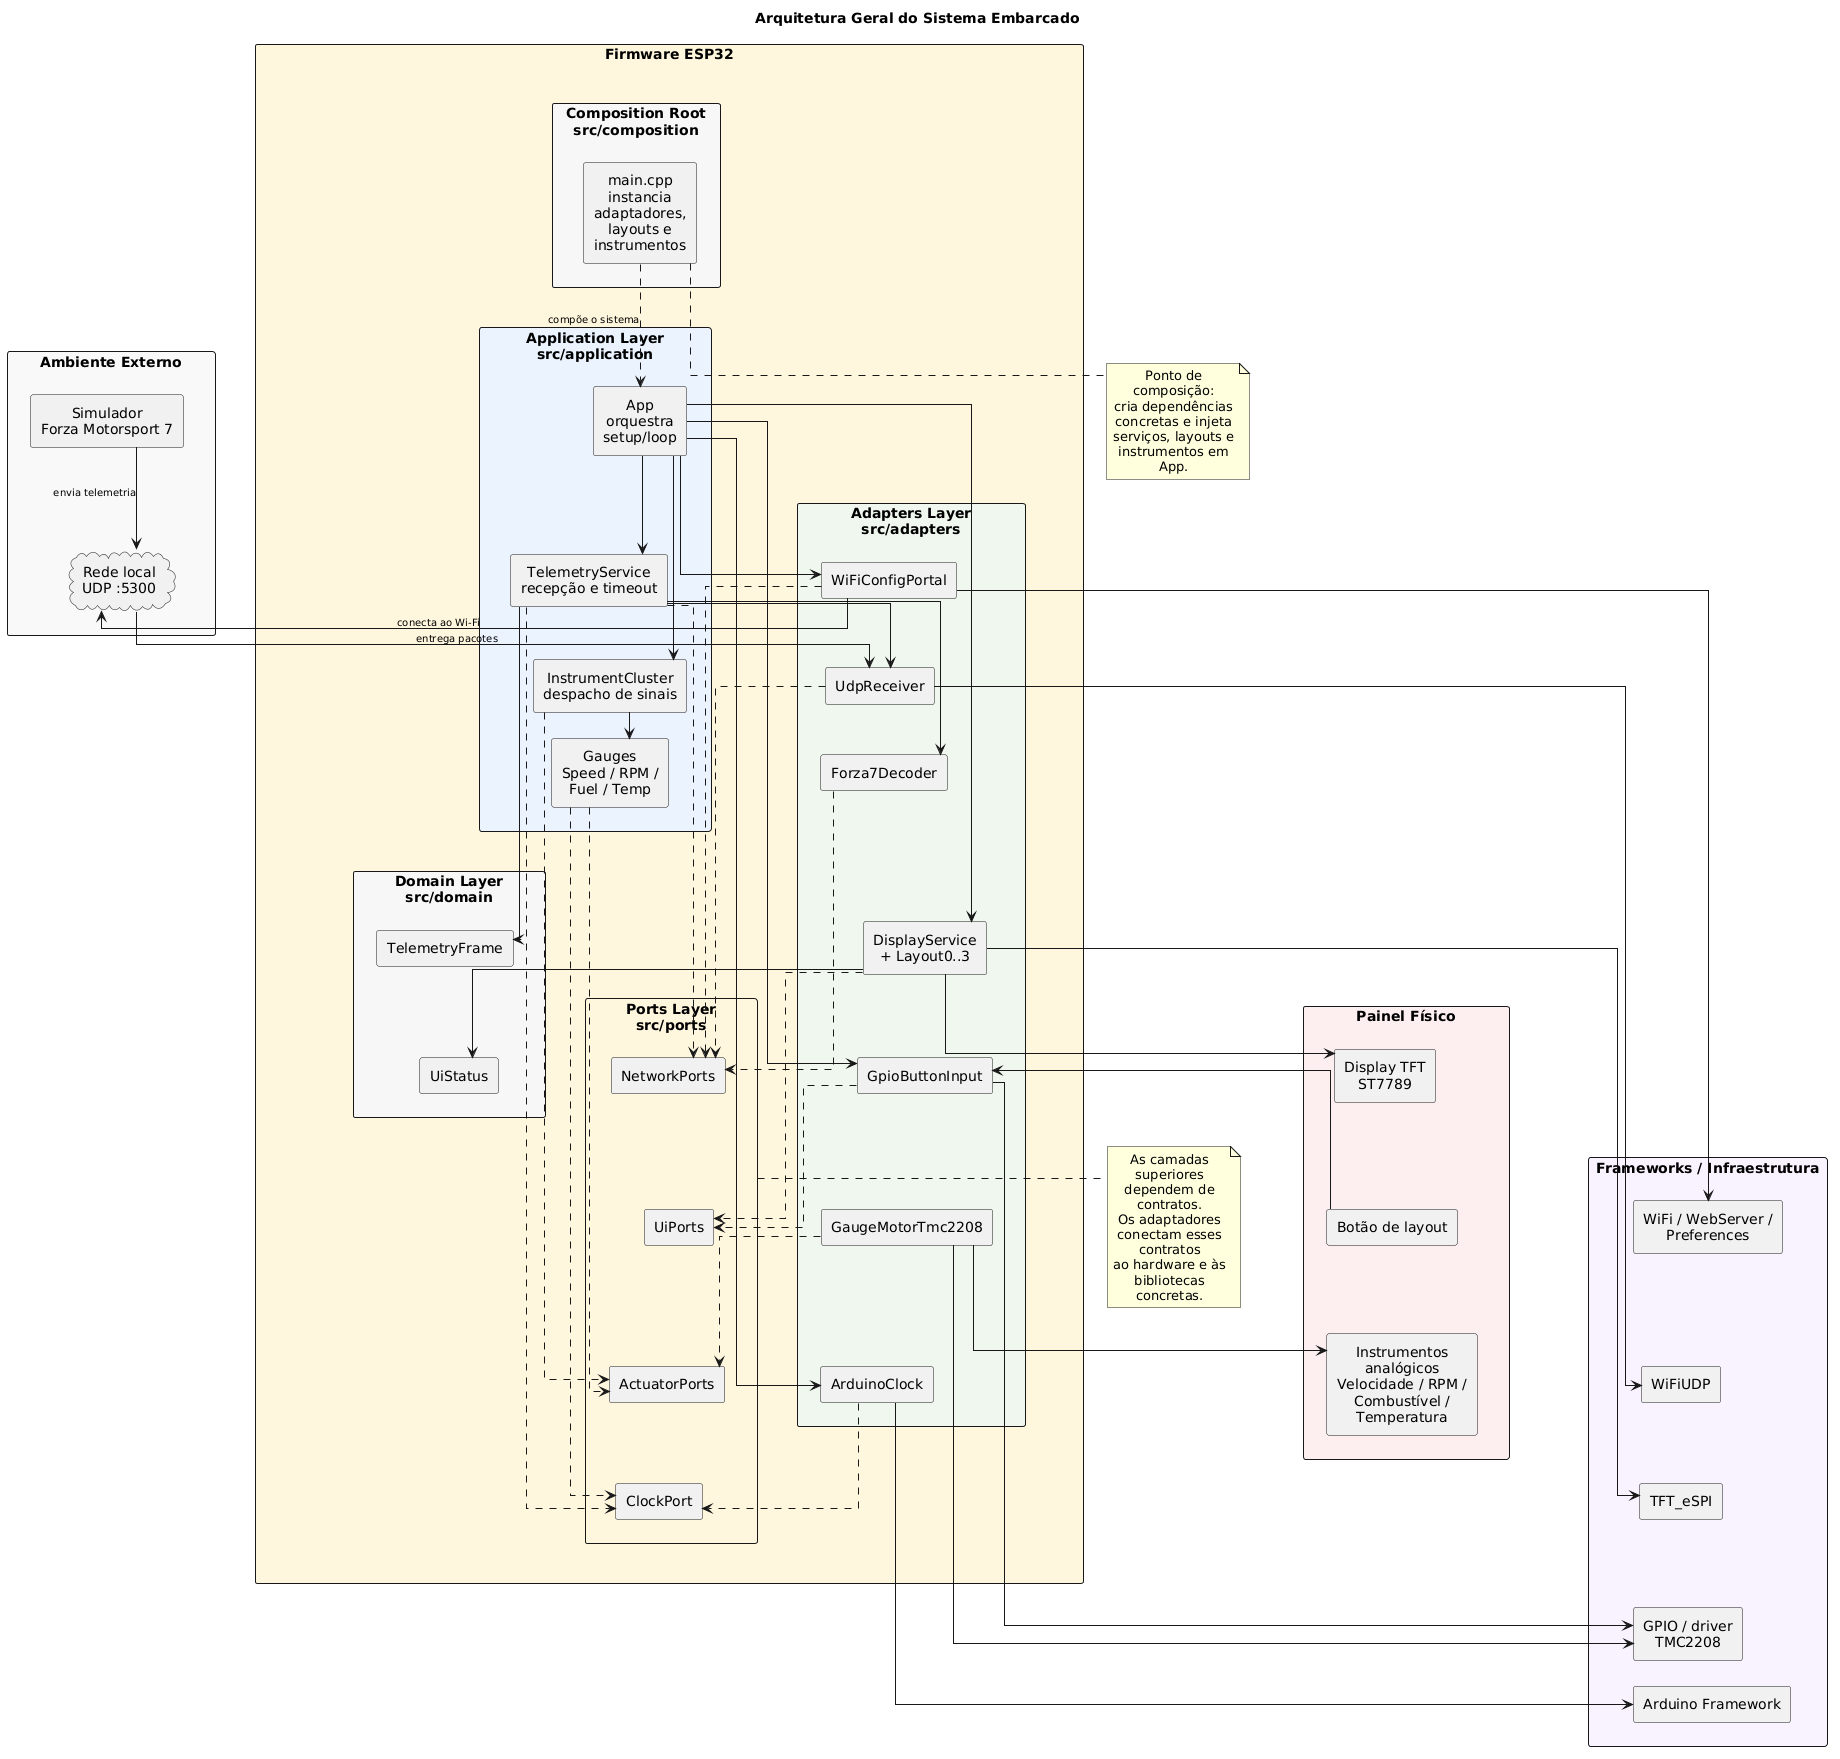
\includegraphics[width=\textwidth]{arquitetura-geral.png}

\par\vspace{4pt}
\noindent\makebox[\textwidth][l]{%
  \fontsize{10pt}{12pt}\selectfont
Fonte: Elaborada pelos autores (2026).%
}

\end{figure}

Na arquitetura geral, o simulador Forza Motorsport 7 envia dados de telemetria pela rede local utilizando pacotes UDP na porta 5300. Esses dados são recebidos pelo \estrangeirismo{firmware} embarcado no ESP32, processados pela aplicação e convertidos em respostas no painel físico, incluindo a movimentação dos instrumentos analógicos e a atualização da interface visual no \estrangeirismo{display} TFT.

A representação arquitetural não detalha classes individuais, pois essa responsabilidade é assumida pelo diagrama de classes apresentado posteriormente. Seu papel é demonstrar como os principais blocos do sistema se relacionam em nível macro: o simulador como fonte dos dados, a rede local como meio de comunicação, o ESP32 como unidade de processamento, os recursos de infraestrutura como suporte operacional e o painel físico como meio de saída perceptível ao usuário.

Essa separação evita a repetição entre os modelos. A arquitetura geral descreve a integração do sistema com o ambiente externo, o diagrama de atividades apresenta o fluxo operacional do sistema, o diagrama de classes descreve a estrutura interna do \estrangeirismo{firmware} e os diagramas de sequência detalham o comportamento temporal das principais operações.


\section{DIAGRAMA DE ATIVIDADES}

Após a apresentação da arquitetura geral, a modelagem comportamental do sistema é detalhada por meio do diagrama de atividades. Segundo \citeonline{sommerville2019}, este diagrama é útil para ilustrar o fluxo de processamento de dados e a sequência de atividades operacionais necessárias para concluir um fluxo de trabalho, evidenciando pontos de decisão, processamentos paralelos, desvios condicionais e interações sequenciais de controle.

No contexto deste projeto, o diagrama de atividades representa o ciclo operacional do \estrangeirismo{firmware} desde o momento em que o hardware é energizado até a execução contínua das rotinas de conectividade, recepção de telemetria, atualização dos instrumentos e supervisão do sistema, conforme ilustrado na Figura~\ref{fig:diagrama_atividades}.

\begin{figure}[!htbp]
\centering
\begin{minipage}{0.95\textwidth}
\centering
\captionsetup{
  width=\linewidth,
  justification=centering,
  singlelinecheck=true,
  font=normalsize
}
\caption{Diagrama de atividades do sistema.}
\label{fig:diagrama_atividades}

\includegraphics[
  width=\linewidth,
  height=0.75\textheight,
  keepaspectratio
]{imagens/diagrama-de-atividades.png}

\par\vspace{4pt}
{\raggedright\fontsize{10pt}{12pt}\selectfont
Fonte: Elaborada pelos autores (2026).\par}

\end{minipage}
\end{figure}
\FloatBarrier % <--- ISSO IMPEDE QUE O TEXTO ABAIXO SEJA IMPRESSO ANTES DA IMAGEM

O fluxo representado é estruturado em três macroblocos principais de execução sequencial:

\begin{itemize}
    \item \textbf{Inicialização:} Compreende o ponto de partida do sistema, realizando a inicialização física e lógica do hardware, a configuração dos componentes de software principais e a verificação inicial das credenciais de rede armazenadas no dispositivo.
    
    \item \textbf{Conexão Wi-Fi:} Gerencia o estado de conectividade de forma condicional. Se o dispositivo já se conecta automaticamente à rede, o fluxo prossegue diretamente. Caso contrário, o \estrangeirismo{firmware} ativa o portal de configuração Wi-Fi e entra em um ciclo de interação: exibe as orientações de configuração no painel, recebe as credenciais submetidas pelo usuário e tenta efetuar a conexão com a rede local até que o acesso seja estabelecido com sucesso.
    
    \item \textbf{Modo Operacional:} Consiste no loop de execução principal da aplicação, subdividido em dois módulos que rodam continuamente enquanto o sistema estiver ativo:
    \begin{itemize}
        \item \textbf{Telemetria:} Responsável por receber os pacotes via rede UDP, validar sua integridade e decodificar os dados brutos. Havendo telemetria válida, o sistema atualiza as variáveis internas de estado, aciona os instrumentos físicos (ponteiros analógicos) e atualiza a interface visual do display TFT. Caso os dados recebidos sejam inválidos (ou em caso de ausência de pacotes), o fluxo desvia para o tratamento de descarte ou erro de sinal, preservando as telas de supervisão do sistema.
        \item \textbf{Interação e Supervisão:} Responsável por escutar interações físicas do usuário. Caso o botão físico seja pressionado, o \estrangeirismo{firmware} alterna ciclicamente o layout ativo da interface TFT. Em seguida, monitora de forma contínua a integridade da conexão Wi-Fi e o estado geral do sistema antes de reiniciar o ciclo de recepção.
    \end{itemize}
\end{itemize} % <--- Este fechamento crucial estava faltando!

\section{DIAGRAMA DE CLASSES}

A Figura~\ref{fig:diagrama_classes} apresenta a visão estrutural principal do \estrangeirismo{firmware}. Diferentemente da arquitetura geral, que descreve a integração entre o simulador, a rede, o ESP32 e o painel físico, o diagrama de classes concentra-se na organização interna do software, evidenciando a classe orquestradora \texttt{App}, os serviços de aplicação, os modelos de domínio, os contratos de porta e os adaptadores concretos de infraestrutura.

\begin{figure}[H]
\centering
\captionsetup{
  width=\textwidth,
  justification=centering,
  singlelinecheck=true,
  font=normalsize
}
\caption{Diagrama de classes do \estrangeirismo{firmware}.}
\label{fig:diagrama_classes}

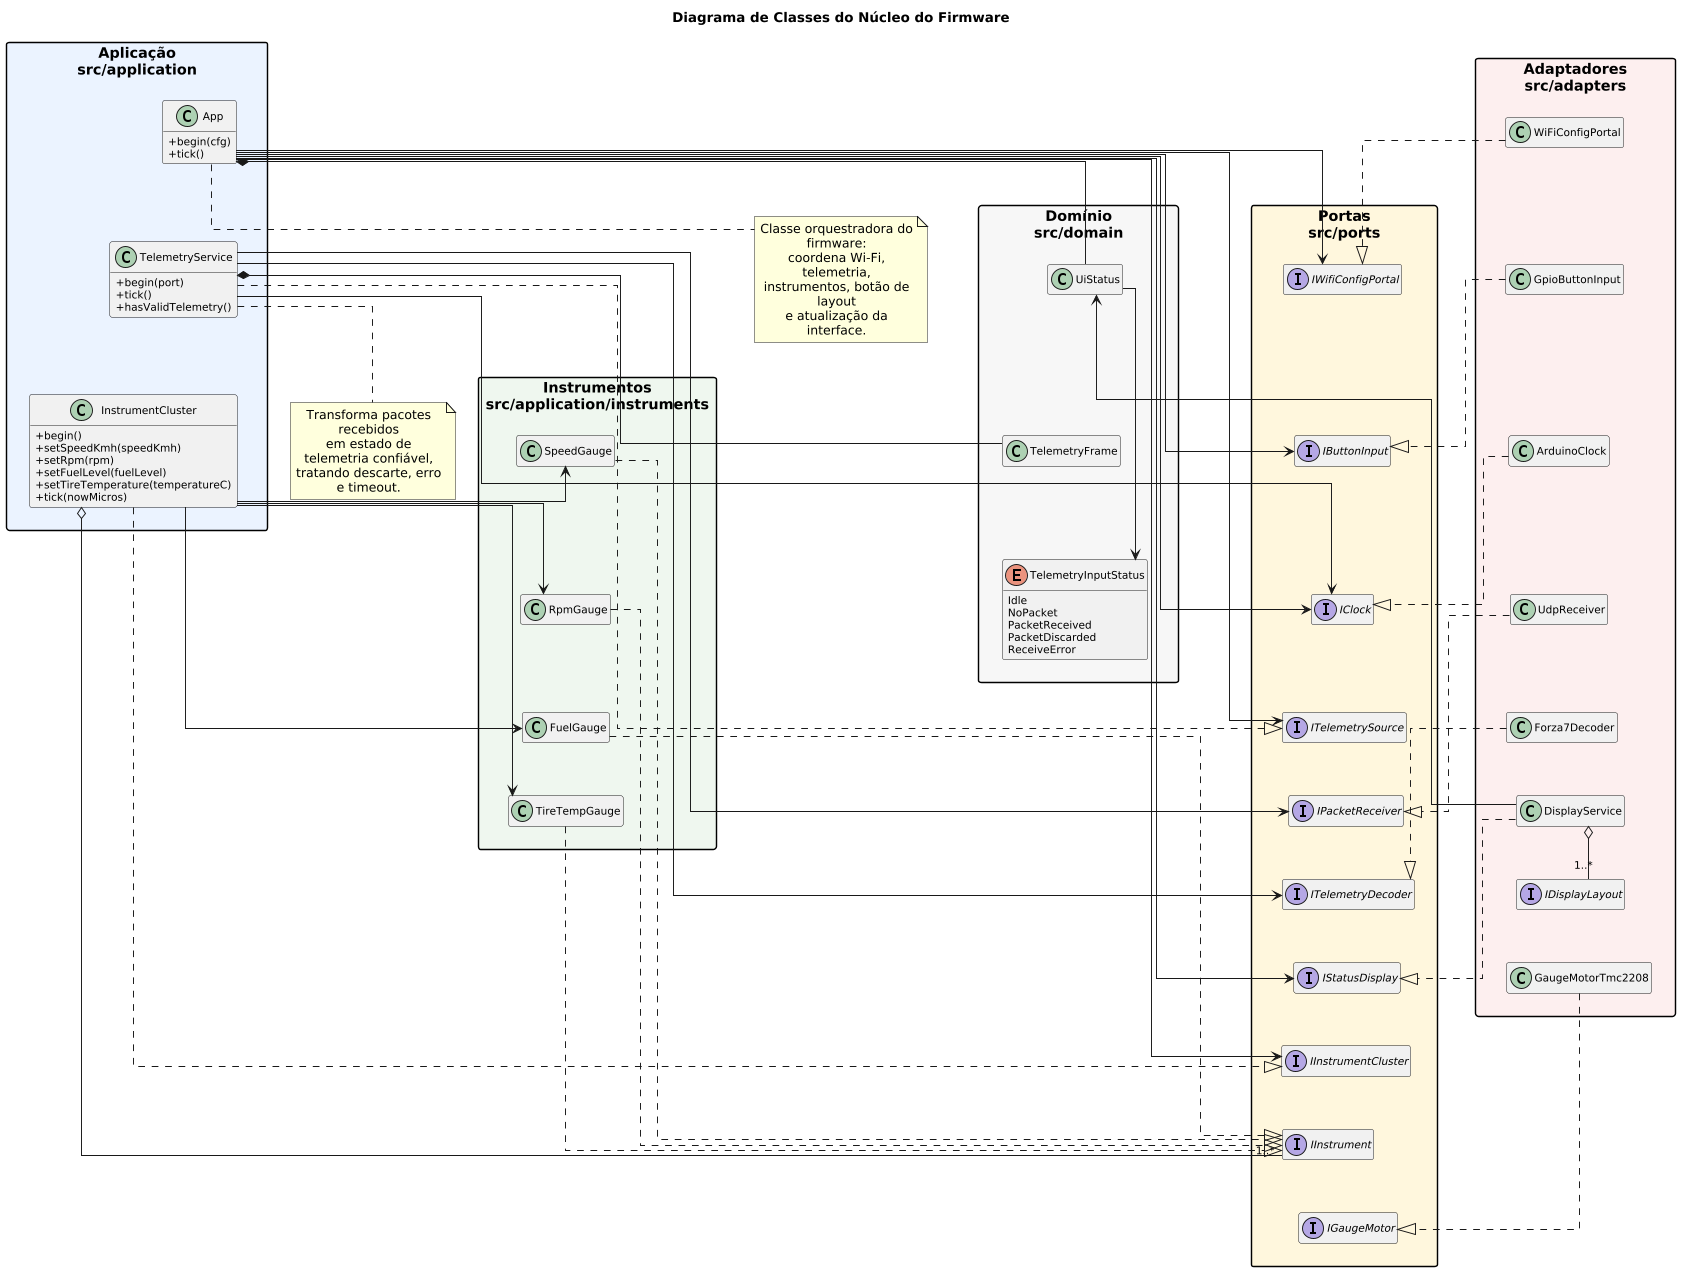
\includegraphics[width=\textwidth]{diagrama-de-classes.png}

\par\vspace{4pt}
\noindent\makebox[\textwidth][l]{%
  \fontsize{10pt}{12pt}\selectfont
  Fonte: Elaborada pelos autores (2026).%
}

\end{figure}

Do ponto de vista de responsabilidade, a classe \texttt{App} coordena o ciclo de vida do sistema; o \texttt{TelemetryService} transforma a entrada de rede em estado de telemetria confiável; o \linebreak\texttt{InstrumentCluster} despacha os valores tratados para instrumentos especializados; e o \texttt{DisplayService} consolida a renderização dos \estrangeirismo{layouts} do painel. A modelagem também evidencia o uso de interfaces como \texttt{IPacketReceiver}, \texttt{ITelemetryDecoder},\linebreak \texttt{IGaugeMotor}, \texttt{IStatusDisplay} e \texttt{IWifiConfigPortal}, decisão central para reduzir acoplamento e favorecer a testabilidade do projeto.

\subsection{EXTENSIBILIDADE PARA NOVOS JOGOS E ATUADORES}

A organização estrutural apresentada no diagrama de classes também evidencia um objetivo de projeto que extrapola o MVP atual: a possibilidade de expansão controlada do sistema para novos jogos e novos elementos de saída física. Essa expansibilidade decorre da separação entre contratos e implementações concretas. No fluxo atual, a origem dos dados do jogo é abstraída por portas de telemetria, enquanto os mecanismos de atuação física são desacoplados da aplicação por contratos próprios de instrumento e acionamento.

Para novos jogos, o principal ponto de extensão está no decodificador de telemetria. Como a aplicação consome um modelo neutro de dados e não depende diretamente do formato bruto dos pacotes, a inclusão de outro simulador pode ser feita por meio de um novo adaptador compatível com o contrato \texttt{ITelemetryDecoder}. Nessa abordagem, o novo jogo passa a ser incorporado sem necessidade de reestruturar a lógica principal da aplicação, desde que os dados relevantes sejam traduzidos para o quadro comum utilizado pelo sistema.

Para novos atuadores, a expansão ocorre de maneira semelhante. O \texttt{Instrument-\linebreak Cluster} já atua como despachante de sinais para classes especializadas que implementam o contrato \texttt{IInstrument}. Isso significa que um novo dispositivo físico pode ser incorporado como mais um consumidor dos sinais da aplicação, preservando a lógica central já existente. Quando o novo atuador puder responder a uma grandeza já disponível no sistema, a adaptação tende a ser localizada. Quando a nova resposta física depender de um evento ainda não representado no domínio, a evolução requerida concentra-se na introdução do novo sinal e em seu encaminhamento pelos contratos correspondentes, sem descaracterizar a arquitetura adotada.
\section{DIAGRAMAS DE SEQUÊNCIA}

Segundo \citeonline{sommerville2019}, os diagramas de sequência são ferramentas fundamentais da modelagem dinâmica de sistemas, pois ilustram a ordem temporal em que os objetos interagem e trocam mensagens para concluir uma tarefa. Para abranger o ciclo de vida da aplicação deste projeto de forma clara, a modelagem desse fluxo foi dividida em três cenários principais: inicialização, operação da rede e processamento da telemetria.

A Figura~\ref{fig:sequencia_inicializacao} ilustra a rotina de inicialização (\estrangeirismo{boot}) do \estrangeirismo{firmware}. Nesta etapa, a classe orquestradora aciona os serviços base e tenta estabelecer conectividade. Se as credenciais de rede não estiverem disponíveis ou falharem, o sistema levanta o portal Wi-Fi de configuração. Após o sucesso da rede, os periféricos (TFT e motores) são instanciados e preparados para uso.

\begin{figure}[H]
\centering
\begin{minipage}{0.9\textwidth}
\centering
\captionsetup{
  width=\linewidth,
  justification=centering,
  singlelinecheck=true,
  font=normalsize
}
\caption{Diagrama de sequência da inicialização do \estrangeirismo{firmware}.}
\label{fig:sequencia_inicializacao}

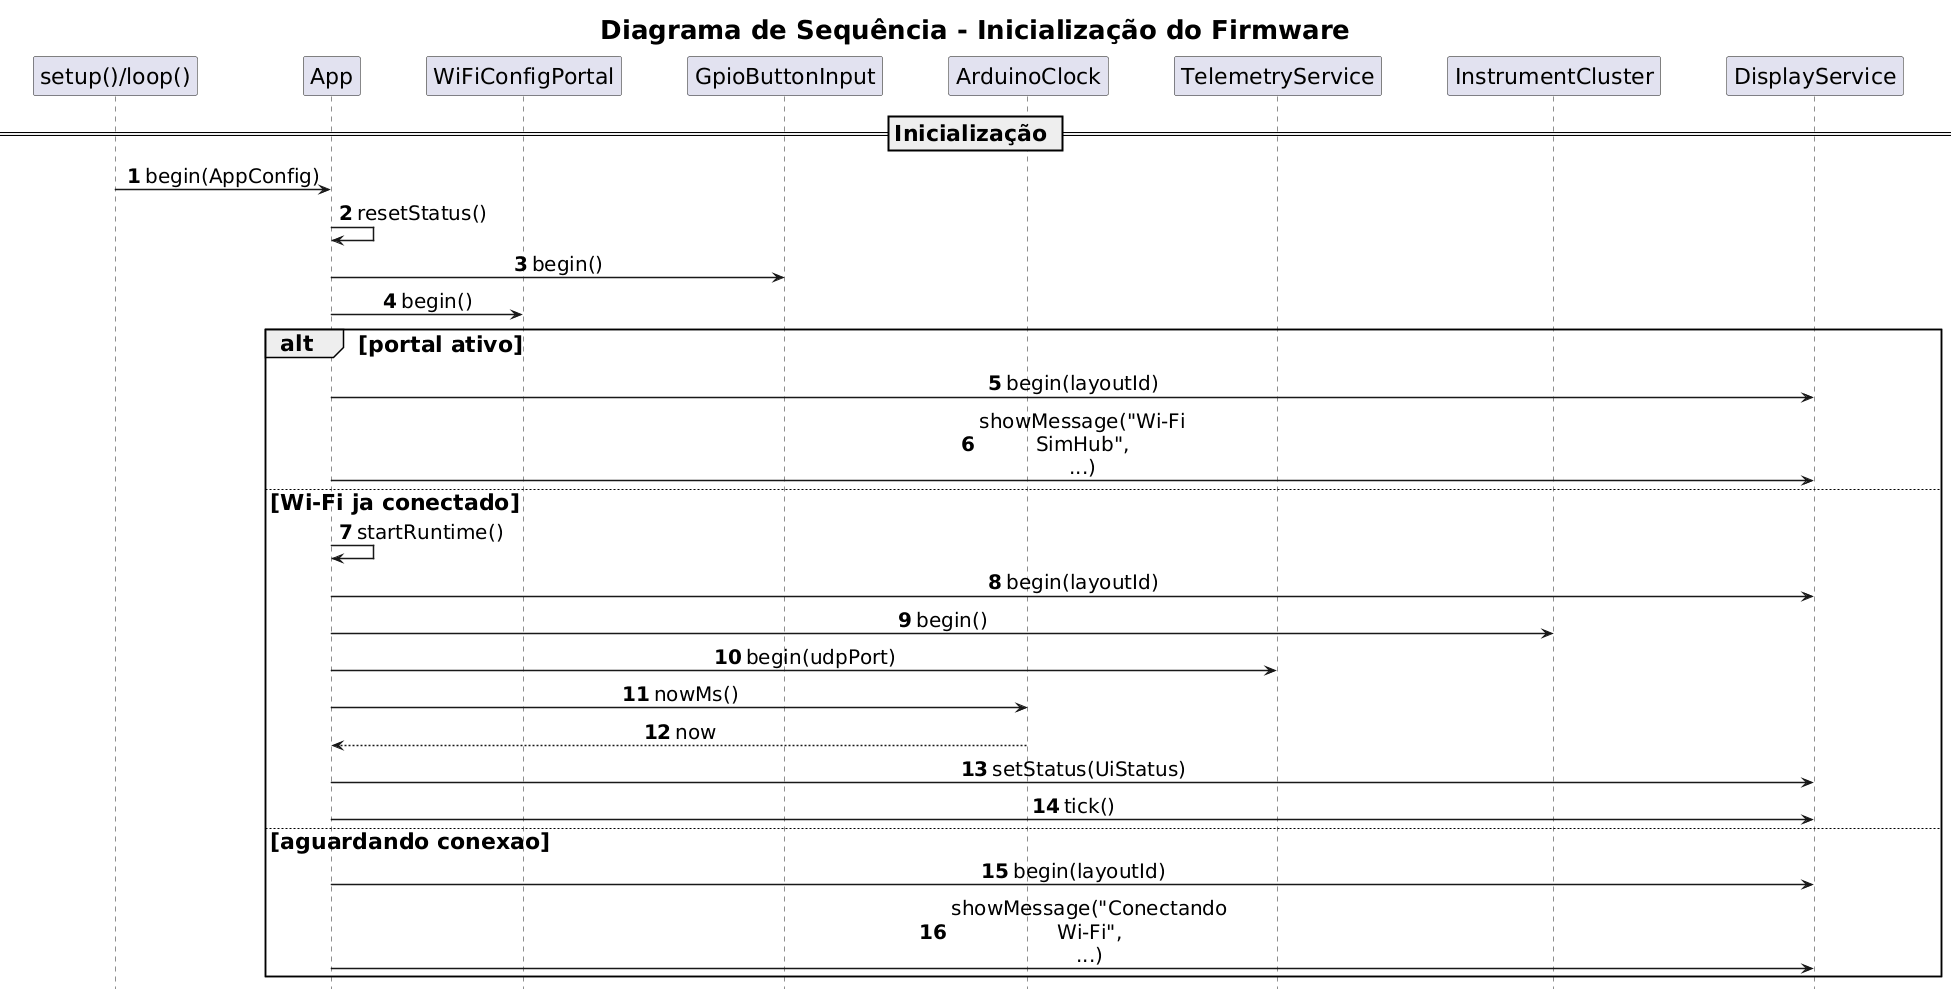
\includegraphics[width=\linewidth]{diagrama-sequencia-inicializacao.png}

\par\vspace{4pt}
{\raggedright\fontsize{10pt}{12pt}\selectfont
Fonte: Elaborada pelos autores (2026).\par}

\end{minipage}
\end{figure}

Uma vez inicializado, o sistema entra em seu fluxo contínuo de operação, conforme detalhado na Figura~\ref{fig:sequencia_operacao_principal}. O \estrangeirismo{loop} principal é responsável por manter a conexão ativa e escutar a porta UDP. Quando o adaptador de rede detecta a chegada de um datagrama, ele captura o pacote e o delega para processamento.

\begin{figure}[H]
\centering
\begin{minipage}{0.95\textwidth}
\centering
\captionsetup{
  width=\linewidth,
  justification=centering,
  singlelinecheck=true,
  font=normalsize
}
\caption{Diagrama de sequência da operação principal do \estrangeirismo{firmware}.}
\label{fig:sequencia_operacao_principal}

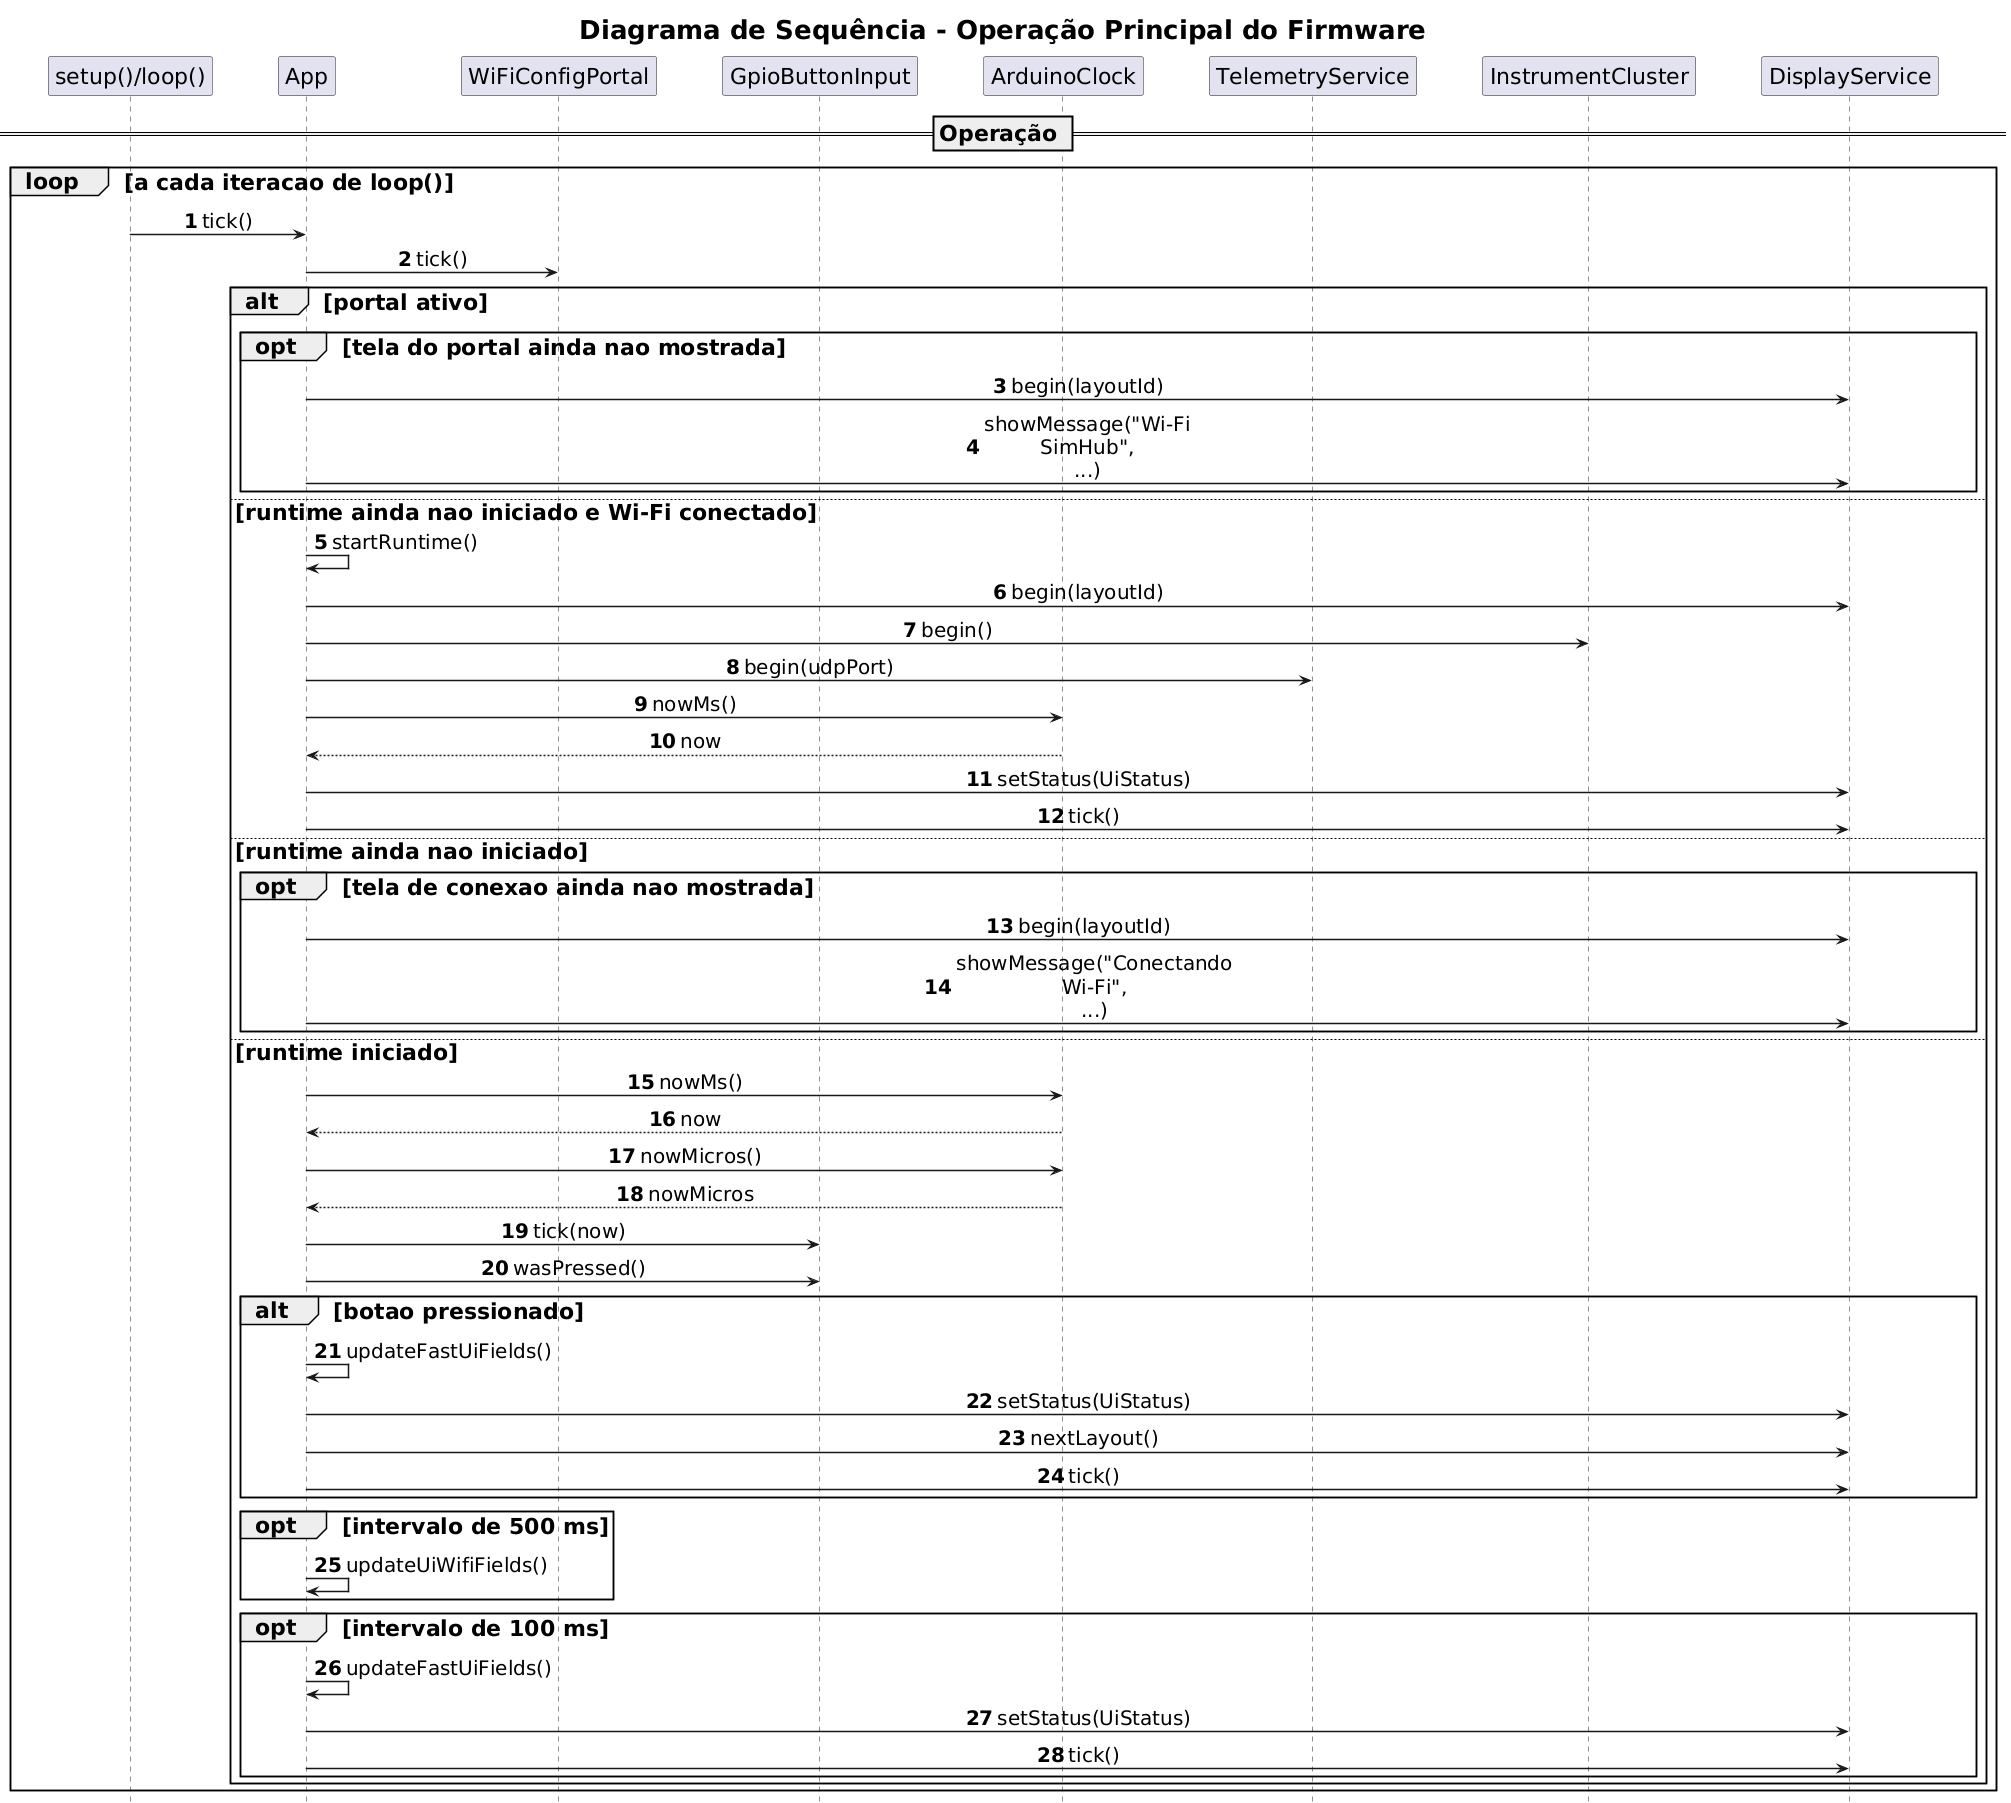
\includegraphics[width=\linewidth]{diagrama-sequencia-operacao-principal.png}

\par\vspace{4pt}
{\raggedright\fontsize{10pt}{12pt}\selectfont
Fonte: Elaborada pelos autores (2026).\par}

\end{minipage}
\end{figure}

Por fim, a Figura~\ref{fig:sequencia_telemetria} demonstra o fluxo interno de conversão dos dados brutos em ações físicas perceptíveis. O pacote UDP recebido é submetido ao decodificador específico do jogo (\texttt{Forza7Decoder}), que extrai os \estrangeirismo{bytes} e os consolida em um modelo padronizado neutro \linebreak(\texttt{TelemetryFrame}). Esse quadro é então despachado em duas frentes: para o \texttt{Instru-\linebreak mentCluster}, que calcula os passos do motor de passo e movimenta os ponteiros analógicos, e para o \texttt{DisplayService}, que atualiza a marcha, velocidade e afins na interface gráfica em tempo real.

\begin{figure}[H]
\centering
\begin{minipage}{0.95\textwidth}
\centering
\captionsetup{
  width=\linewidth,
  justification=centering,
  singlelinecheck=true,
  font=normalsize
}
\caption{Diagrama de sequência de telemetria e instrumentos.}
\label{fig:sequencia_telemetria}

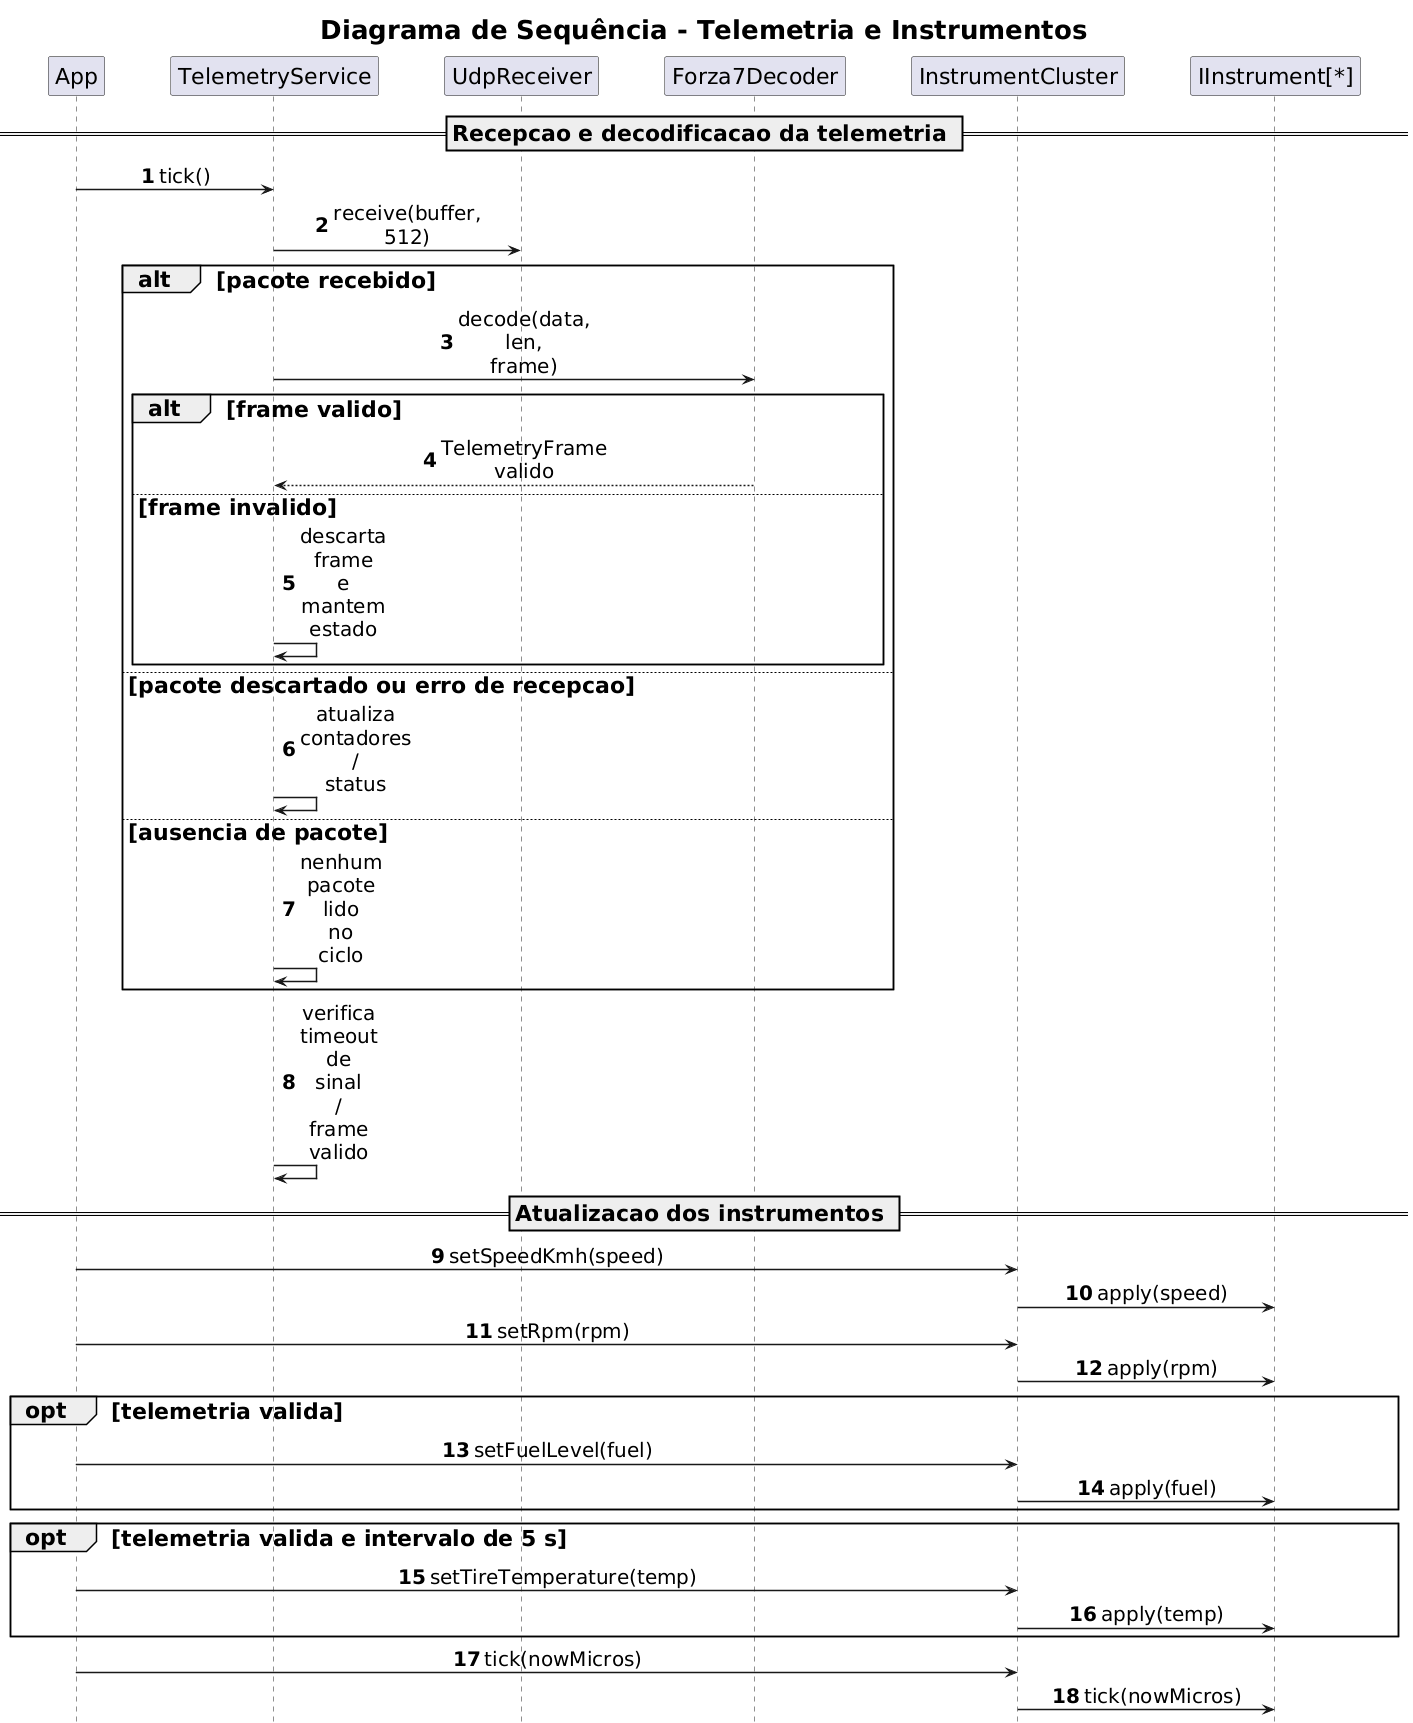
\includegraphics[width=\linewidth]{diagrama-sequencia-telemetria.png}

\par\vspace{4pt}
{\raggedright\fontsize{10pt}{12pt}\selectfont
Fonte: Elaborada pelos autores (2026).\par}

\end{minipage}
\end{figure}

\section{INTERFACES}

A interface do sistema é inteiramente embarcada e se divide em dois contextos: mensagens de estado operacional e \estrangeirismo{layouts} de telemetria exibidos no \estrangeirismo{display} TFT. O projeto visual prioriza a legibilidade e o contraste, garantindo que o piloto identifique informações críticas de forma instantânea. As especificações de cada \estrangeirismo{layout} implementado estão consolidadas no Quadro~\ref{quad:interfaces}.

\begin{quadro}[H]
\centering
\captionsetup{
  width=\textwidth,
  justification=centering,
  singlelinecheck=true,
  font=normalsize,
  labelfont=normalfont,
  textfont=normalfont
}
\caption{Interfaces visuais implementadas no \estrangeirismo{display}}
\label{quad:interfaces}

{\fontsize{10pt}{12pt}\selectfont
\renewcommand{\arraystretch}{1.25}
\setlength{\tabcolsep}{6pt}
\begin{tabularx}{\textwidth}{|
  >{\raggedright\arraybackslash}p{3.0cm}|
  >{\raggedright\arraybackslash}X|
}
\hline
\textbf{Interface} & \textbf{Conteúdo principal} \\
\hline
\texttt{Layout0Basic} & Exibe posição de corrida, volta atual e marcha em destaque, privilegiando leitura rápida de estado competitivo. \\
\hline
\texttt{Layout1Minimal} & Exibe marcha central, velocidade, RPM e percentual de combustível, servindo como painel sintético geral. \\
\hline
\texttt{Layout2Performance} & Exibe velocidade ampliada, marcha, combustível com codificação por cor e barra de RPM. \\
\hline
\texttt{Layout3Tires} & Exibe temperaturas individuais \texttt{FL}, \texttt{FR}, \texttt{RL} e \texttt{RR} com codificação cromática por faixa térmica. \\
\hline
Telas de estado & Apresentam mensagens de conexão, orientação para acesso ao portal \texttt{SimHub} e aguardam configuração ou estabelecimento de rede. \\
\hline
\end{tabularx}
}

\par\vspace{4pt}
\noindent\makebox[\textwidth][l]{%
  \fontsize{10pt}{12pt}\selectfont
  Fonte: Elaborada pelos autores (2026).%
}

\end{quadro}

A navegação entre os contextos é realizada por um botão físico ligado ao pino 16. O \estrangeirismo{display} opera com resolução de 240x320 pixels sob o controlador ST7789. As capturas de tela a seguir ilustram a implementação real de cada interface descrita.

% --- BLOCO PARA AS IMAGENS DAS TELAS ---

\begin{figure}[!htbp]
\centering
\begin{minipage}{0.95\textwidth}
\centering
\captionsetup{
  width=\linewidth,
  justification=centering,
  singlelinecheck=true,
  font=normalsize
}
\caption{Interface de telemetria: Layout0Basic e Layout1Minimal.}
\label{fig:layouts_iniciais}

\includegraphics[width=0.47\linewidth]{imagens/layout0.png}
\hfill
\includegraphics[width=0.47\linewidth]{imagens/layout1.png}

\par\vspace{4pt}
{\raggedright\fontsize{10pt}{12pt}\selectfont
Fonte: Elaborada pelos autores (2026).\par}

\end{minipage}
\end{figure}
\begin{figure}[!htbp]
\centering
\begin{minipage}{0.95\textwidth}
\centering
\captionsetup{
  width=\linewidth,
  justification=centering,
  singlelinecheck=true,
  font=normalsize
}
\caption{Interface de telemetria: Layout2Performance e Layout3Tires.}
\label{fig:layouts_performance}

\includegraphics[width=0.47\linewidth]{imagens/layout2.png}
\hfill
\includegraphics[width=0.47\linewidth]{imagens/layout3.png}

\par\vspace{4pt}
{\raggedright\fontsize{10pt}{12pt}\selectfont
Fonte: Elaborada pelos autores (2026).\par}

\end{minipage}
\end{figure}
\begin{figure}[!htbp]
\centering
\begin{minipage}{0.95\textwidth}
\centering
\captionsetup{
  width=\linewidth,
  justification=centering,
  singlelinecheck=true,
  font=normalsize
}
\caption{Telas de estado e inicialização do sistema.}
\label{fig:telas_estado}

\includegraphics[width=0.47\linewidth]{imagens/tela_conexao.png}
\hfill
\includegraphics[width=0.47\linewidth]{imagens/tela-sucesso-conexao.png}

\par\vspace{4pt}
{\raggedright\fontsize{10pt}{12pt}\selectfont
Fonte: Elaborada pelos autores (2026).\par}

\end{minipage}
\end{figure}
\chapter{SOFTWARE}
\label{sec:software}

Este capítulo apresenta a materialização do software embarcado do projeto, contemplando sua implantação, seu fluxo de execução e a estratégia empregada para validar o \estrangeirismo{firmware} no computador e no ESP32. O objetivo é complementar a modelagem anterior com uma visão mais operacional do produto efetivamente entregue.

\section{IMPLANTAÇÃO}

A implantação do projeto corresponde ao processo de preparação, compilação, gravação e verificação inicial do firmware no ESP32. Essa etapa é importante porque conecta o código-fonte desenvolvido ao funcionamento real do protótipo, permitindo que o sistema seja executado no microcontrolador e validado de forma progressiva.

No projeto, esse processo começa pela preparação do ambiente local, passa pela revisão dos arquivos de configuração, segue para a compilação e gravação do firmware e termina com a execução das suítes de teste previstas. Como parte do fluxo depende de ferramentas instaladas localmente e da organização específica do repositório, os comandos apresentados foram mantidos de acordo com os procedimentos efetivamente utilizados durante o desenvolvimento.

\subsection{PREPARAÇÃO DO AMBIENTE E CONFIGURAÇÕES DO PROJETO}

O primeiro passo consiste em obter o repositório e preparar um ambiente virtual local para as ferramentas de desenvolvimento. Esse arranjo reproduz o fluxo utilizado nas execuções documentadas do projeto e atende também ao script de cobertura, que procura o executável do \texttt{gcovr} dentro de \texttt{./.venv}. Um roteiro funcional é apresentado a seguir:

\begin{verbatim}
git clone https://github.com/CaironFerreira/TCC
cd TCC
python3 -m venv .venv
source .venv/bin/activate
pip install platformio gcovr
export PLATFORMIO_CORE_DIR=$PWD/.platformio-core
./.venv/bin/platformio --version
\end{verbatim}

Nos exemplos seguintes, adota-se o executável \texttt{./.venv/bin/platformio}. Quando o atalho \texttt{pio} já estiver disponível no PATH, ele pode ser utilizado como equivalente. Além do ambiente Python, a máquina precisa dispor de compilador C/C++ funcional. Para a medição de cobertura registrada neste trabalho, o script \texttt{./scripts/run\_native\_coverage.sh} foi preparado para macOS e utiliza \texttt{xcrun llvm-cov gcov}.

Antes da compilação, também é necessário revisar os arquivos \texttt{include/User\_Setup.h} e \texttt{src/config/BoardConfig.h}. O arquivo \texttt{include/User\_Setup.h} concentra a configuração do display ST7789, enquanto o arquivo \texttt{src/config/BoardConfig.h} define parâmetros diretamente relacionados ao funcionamento do protótipo, como porta UDP, botão de troca de layout, pinos dos motores, escalas e limites lógicos dos instrumentos.

Essa verificação é necessária porque o build pode ser concluído com sucesso mesmo quando a pinagem física do protótipo não corresponde às definições presentes no código. Assim, a revisão dos arquivos de configuração evita que problemas de montagem ou parametrização sejam interpretados incorretamente como falhas de implementação.

\subsection{COMPILAÇÃO, GRAVAÇÃO E PRIMEIRA EXECUÇÃO}

Com o ambiente preparado e os arquivos de configuração revisados, a próxima etapa é compilar o firmware principal. O ambiente embarcado de produção está definido em \texttt{platformio.ini} como \texttt{esp32dev}. A compilação pode ser realizada com:

\begin{verbatim}
./.venv/bin/platformio run -e esp32dev
\end{verbatim}

Na primeira execução, o PlatformIO pode levar mais tempo, pois precisa baixar a plataforma \texttt{espressif32}, preparar a cadeia de compilação do microcontrolador e instalar a dependência \texttt{TFT\_eSPI}. Após a conclusão do build, a gravação do binário na placa pode ser feita com:

\begin{verbatim}
./.venv/bin/platformio run -e esp32dev -t upload
\end{verbatim}

Depois do upload, o comportamento do dispositivo pode ser acompanhado pelo monitor serial configurado a 115200 bps:

\begin{verbatim}
./.venv/bin/platformio device monitor -b 115200
\end{verbatim}

O monitor serial não é obrigatório para a gravação do programa, mas auxilia na observação de mensagens de estado, reinicializações, tentativas de conexão e possíveis falhas durante os ensaios embarcados.

Com o firmware gravado, o dispositivo tenta reutilizar credenciais de rede previamente salvas. Se a conexão for bem-sucedida, o protótipo entra no modo operacional e passa a aguardar telemetria na porta UDP 5300. Em caso de falha, o ESP32 ativa o ponto de acesso \texttt{SimHub}, sem senha, e o display orienta o usuário a abrir \texttt{http://simhub} para informar o SSID e a senha da rede local.

Após a conexão Wi-Fi, o simulador deve ser configurado para enviar telemetria no formato Forza Motorsport 7 Data Out para o endereço IP do ESP32 na mesma rede local e na porta UDP 5300. A partir daí, o \texttt{UdpReceiver} recebe os pacotes, o \texttt{Forza7Decoder} extrai os campos relevantes e o \texttt{TelemetryService} distribui os valores processados para a interface visual e para os instrumentos físicos.

\subsection{VALIDAÇÃO DA IMPLANTAÇÃO POR TESTES}

A validação da implantação foi organizada de forma incremental. Primeiro, executam-se os testes no ambiente host-side, sem depender do ESP32 conectado. Em seguida, realiza-se o smoke test embarcado. Por fim, quando as condições de bancada permitem, executa-se a integração UDP real no microcontrolador. Essa sequência reduz o risco de iniciar a validação diretamente pelo hardware sem antes verificar o núcleo lógico do firmware.

O primeiro comando a ser executado é:

\begin{verbatim}
./.venv/bin/platformio test -e test_native
\end{verbatim}

Esse ambiente reúne as suítes unitárias, de integração host-side e de componente. Ele não depende do ESP32 conectado e serve para validar o núcleo do firmware. Sua primeira execução também faz o PlatformIO baixar o framework Unity em \texttt{.pio/libdeps/test\_native/}, dependência utilizada posteriormente pelo script de cobertura.

Depois da aprovação do ambiente \texttt{test\_native}, recomenda-se executar o teste embarcado mais simples:

\begin{verbatim}
./.venv/bin/platformio test -e test_esp32_smoke
\end{verbatim}

Esse comando compila a suíte de smoke, envia o binário de teste para o ESP32 e coleta o resultado pela serial. Seu objetivo é confirmar que o fluxo principal da aplicação inicia no microcontrolador e executa corretamente o caminho básico previsto pela suíte.

A etapa seguinte corresponde à integração UDP real:

\begin{verbatim}
./.venv/bin/platformio test -e test_esp32_udp_integration
\end{verbatim}

Esse ambiente ativa Wi-Fi real no ESP32, cria o ponto de acesso \texttt{TCC-Test}, envia pacotes UDP reais para o \texttt{UdpReceiver} e verifica o comportamento conjunto de \texttt{WiFiUDP}, \linebreak\texttt{Forza7Decoder} e \texttt{TelemetryService}. A documentação do projeto registra, contudo, uma limitação objetiva dessa etapa: com alimentação exclusivamente via USB, o protótipo pode entrar em \texttt{brownout} durante a ativação do rádio.

Por fim, a cobertura de código consolidada pode ser reproduzida com:

\begin{verbatim}
./scripts/run_native_coverage.sh
\end{verbatim}

Embora exista um ambiente \texttt{test\_native\_coverage} no \texttt{platformio.ini}, a medição consolidada registrada neste trabalho é gerada pelo script acima. Para que ele funcione corretamente, o ambiente virtual deve existir com \texttt{gcovr} instalado e o comando \texttt{./.venv/bin/platformio test -e test\_native} deve ter sido executado ao menos uma vez, de modo que a dependência Unity esteja presente em \texttt{.pio/libdeps/test\_native/}. A saída esperada é a geração de relatórios em \texttt{coverage/reports/}.

Assim, a implantação completa do projeto corresponde a um ciclo técnico verificável: preparar o ambiente, revisar as configurações do protótipo, compilar, gravar o firmware e validar seu comportamento no computador e no microcontrolador.

\section{IMPLEMENTAÇÃO DO FIRMWARE}

A implementação do \estrangeirismo{firmware} concretiza, no código-fonte, a arquitetura definida na etapa de modelagem. O sistema foi organizado de modo a separar responsabilidades entre recepção de dados, decodificação da telemetria, coordenação da aplicação, exibição visual, acionamento dos instrumentos físicos e gerenciamento da conectividade sem fio. Essa divisão favorece a manutenção do código, facilita a substituição de componentes específicos e reduz o acoplamento direto entre regras de aplicação e detalhes de \estrangeirismo{hardware}.

No contexto do projeto, o \estrangeirismo{firmware} não atua apenas como um leitor de pacotes UDP. Ele coordena um fluxo contínuo em que dados produzidos pelo simulador são recebidos, interpretados, normalizados e transformados em respostas visuais e físicas no painel. Assim, a implementação precisa lidar simultaneamente com comunicação de rede, atualização de interface, acionamento mecânico, persistência de credenciais e controle de estados de operação.

\subsection{COMPOSIÇÃO, INICIALIZAÇÃO E CICLO DE EXECUÇÃO}

O ponto de composição do \estrangeirismo{firmware} encontra-se em \texttt{src/composition/main.cpp}. Nesse arquivo são instanciados e conectados os principais elementos do sistema, incluindo o portal Wi-Fi, o receptor UDP, o decodificador de telemetria, os serviços de aplicação, o \estrangeirismo{display}, os motores e os instrumentos analógicos. Essa concentração da montagem em um único ponto facilita a compreensão da estrutura final do protótipo, pois torna explícito quais componentes participam da aplicação e como eles são associados antes do início da execução.

A composição adotada é majoritariamente estática. Objetos como \texttt{TelemetryService}, \texttt{DisplayService}, \texttt{InstrumentCluster} e \texttt{App} são declarados de forma persistente e ligados antes da entrada nos ciclos principais do ambiente Arduino, representados pelas funções \texttt{setup()} e \texttt{loop()}. Essa estratégia é adequada ao contexto embarcado, pois reduz alocações dinâmicas durante a execução e torna o comportamento do sistema mais previsível em um microcontrolador com recursos limitados.

Nesse mesmo ponto também são organizados dois catálogos centrais para o funcionamento do painel: o conjunto de \estrangeirismo{layouts} disponíveis para o \estrangeirismo{display} e o conjunto de instrumentos físicos reunidos no \texttt{InstrumentCluster}. O primeiro permite alternar diferentes formas de apresentação visual da telemetria, enquanto o segundo centraliza os instrumentos responsáveis por representar fisicamente grandezas como velocidade, rotação, combustível e temperatura. Dessa forma, o arquivo de composição funciona como o local em que a arquitetura abstrata do sistema é efetivamente transformada em uma aplicação executável.

A classe \texttt{App} atua como orquestradora principal do \estrangeirismo{firmware}. Durante a chamada de \linebreak\texttt{begin()}, ela redefine o estado inicial da interface, prepara o botão físico de troca de \estrangeirismo{layout} e aciona o portal Wi-Fi. Nessa etapa, a aplicação diferencia três situações principais: abertura imediata do portal de configuração, entrada direta em modo operacional quando há credenciais válidas ou exibição de uma tela transitória enquanto a conexão é tentada.

Após a inicialização, a rotina \texttt{tick()} passa a conduzir o ciclo contínuo do sistema. A cada iteração, a aplicação atualiza o estado do portal Wi-Fi, verifica a interação do usuário com o botão de troca de telas, aciona o serviço de telemetria, atualiza os instrumentos físicos e repassa periodicamente o estado consolidado ao \estrangeirismo{display}. Esse fluxo garante que o sistema permaneça responsivo tanto à chegada de novos pacotes quanto às ações locais do usuário.

A implementação também diferencia intervalos de atualização para tarefas distintas. A interface visual, a conectividade e o cálculo da temperatura média dos pneus não precisam ser atualizados necessariamente com a mesma frequência. Ao separar esses intervalos, o \estrangeirismo{firmware} evita processamento desnecessário, reduz oscilações visuais e preserva maior estabilidade durante a operação contínua do painel.

\subsection{PIPELINE DE TELEMETRIA E ATUALIZAÇÃO DAS SAÍDAS}

O núcleo funcional do produto está no pipeline formado por \texttt{UdpReceiver}, \texttt{Forza7-Decoder} e \texttt{TelemetryService}. O \texttt{UdpReceiver} é responsável por receber os datagramas UDP enviados pelo simulador; o \texttt{Forza7Decoder} interpreta os dados conforme o formato \estrangeirismo{Forza Motorsport 7 (Data Out)}; e o \texttt{TelemetryService} organiza o resultado da decodificação em valores consumíveis pela aplicação.

Na implementação atual, o \texttt{Forza7Decoder} opera sobre deslocamentos fixos do pacote de telemetria. Essa abordagem é compatível com o formato enviado pelo simulador, no qual cada grandeza relevante ocupa posições conhecidas dentro do datagrama. Além da leitura dos campos, o decodificador já aplica transformações necessárias ao uso prático dos dados, como a conversão da velocidade para quilômetros por hora e o cálculo da temperatura média dos pneus.

O \texttt{TelemetryService} complementa esse processo ao acrescentar controle de estado sobre o fluxo de dados. Entre suas responsabilidades estão a limitação da quantidade de pacotes processados por ciclo, a contagem de descartes e erros, a identificação de presença ou ausência de sinal, a invalidação de dados por \estrangeirismo{timeout} e a normalização dos valores antes do repasse à camada superior. Com isso, a aplicação não depende diretamente da leitura bruta dos pacotes UDP, mas de um estado de telemetria já tratado e coerente para uso no painel.

Depois do processamento, os dados são distribuídos por duas rotas principais: a interface visual e os instrumentos físicos. Na interface, o \texttt{DisplayService} mantém o catálogo de \estrangeirismo{layouts}, inicializa o \estrangeirismo{display} quando necessário e controla a troca de telas conforme a interação do usuário. Cada \estrangeirismo{layout} representa uma forma específica de apresentar a telemetria, permitindo adaptar a visualização às informações mais relevantes em cada contexto de uso.

No plano físico, o \texttt{InstrumentCluster} atua como despachante dos sinais destinados aos instrumentos analógicos. Em vez de a aplicação acionar diretamente cada motor ou cada instrumento, ela encaminha os valores consolidados ao agrupador, que distribui cada grandeza apenas aos instrumentos compatíveis. Essa separação evita que a lógica principal da aplicação fique dependente dos detalhes de acionamento mecânico e preserva a possibilidade de adicionar, remover ou substituir instrumentos com menor impacto sobre o restante do código.

Essa organização é coerente com o objetivo central do projeto: converter a telemetria digital do simulador em uma experiência híbrida, composta por resposta gráfica e resposta física. O \estrangeirismo{firmware}, portanto, não se limita a exibir números em tela, mas transforma os dados recebidos em comportamento perceptível no painel, aproximando o protótipo da experiência de um painel automotivo dedicado.

\subsection{CONECTIVIDADE, PERSISTÊNCIA E SUPORTE OPERACIONAL}

A conectividade sem fio é um elemento essencial da implementação, pois a recepção da telemetria depende de o ESP32 estar conectado à mesma rede do equipamento que executa o simulador. Para reduzir a necessidade de recompilação sempre que o ambiente de rede muda, foi implementado o componente \texttt{WiFiConfigPortal}. Esse componente permite configurar as credenciais de rede por meio de uma interface local, tornando o protótipo mais adequado ao uso prático em diferentes ambientes.

Durante a inicialização, o \texttt{WiFiConfigPortal} procura credenciais previamente persistidas, tenta estabelecer conexão com a rede configurada e, em caso de falha, ativa automaticamente um ponto de acesso de configuração. Nesse modo, o usuário pode acessar a interface web local e informar o SSID e a senha da rede desejada. Após o sucesso da conexão, as credenciais são armazenadas para reutilização em execuções futuras, evitando que o usuário precise repetir o procedimento a cada reinicialização do dispositivo.

Além da abertura do portal de configuração, o componente administra a leitura e gravação de dados em \texttt{Preferences}, diferencia estados de conexão, processa requisições HTTP, encerra o ponto de acesso após a configuração bem-sucedida e mantém tentativas de reaproveitamento das credenciais salvas. Dessa forma, a conectividade deixa de ser tratada como uma configuração fixa inserida no código-fonte e passa a integrar o comportamento operacional do próprio produto.

Esse mecanismo é importante porque o protótipo foi concebido para funcionar como um dispositivo embarcado independente. Em um cenário de uso real, não seria adequado exigir alterações no código ou nova gravação do \estrangeirismo{firmware} sempre que o painel fosse utilizado em outra rede. A presença do portal Wi-Fi, portanto, aproxima o sistema de uma solução mais autônoma e reduz a dependência de intervenção técnica para sua utilização.

\subsection{PONTOS DE EXPANSÃO DO FIRMWARE}

A implementação atual também define pontos de extensão que permitem evoluir o projeto sem reestruturar toda a arquitetura. No caso de suporte a novos jogos, o caminho natural consiste em adicionar um novo par de arquivos em \texttt{src/adapters/telemetry/}, seguindo o padrão do \texttt{Forza7Decoder} e implementando o contrato \texttt{ITelemetryDecoder}. Se o protocolo do novo simulador disponibilizar apenas os campos já contemplados pelo sistema, o novo adaptador pode traduzir diretamente esses dados para o modelo \texttt{TelemetryFrame}.

Caso o novo protocolo ofereça informações adicionais relevantes, a ampliação passa por acrescentar novos campos em \texttt{src/domain/TelemetryFrame.h} e, quando necessário, expô-los também por meio do serviço de telemetria consumido pela aplicação. Após a criação do novo decodificador, sua integração ocorre no ponto de composição principal, em \texttt{src/composition/main-.cpp}, onde atualmente é instanciado o \texttt{Forza7Decoder}. Essa escolha mantém a troca ou adição de suporte a outro jogo concentrada na borda de entrada da arquitetura.

Para preservar a confiabilidade do sistema durante essa evolução, a inclusão de um novo decodificador deve ser acompanhada por testes equivalentes aos existentes para o protocolo atual. Esses testes devem verificar tanto a leitura dos campos do pacote quanto o comportamento integrado do pipeline de telemetria, garantindo que os dados continuem sendo normalizados e distribuídos corretamente à aplicação.

A expansão para novos atuadores segue lógica semelhante. Quando o novo dispositivo puder operar a partir de uma grandeza já tratada pelo sistema, como velocidade, rotação, combustível ou temperatura, basta implementar uma nova classe em \texttt{src/application/instru-\linebreak ments/} compatível com o contrato \texttt{IInstrument} e registrá-la no arranjo do \texttt{Instrument-\linebreak Cluster} em \texttt{src/composition/main.cpp}. Se esse atuador exigir um mecanismo físico de acionamento ainda não contemplado, um adaptador correspondente pode ser acrescentado em \texttt{src/adapters/motors/}, seguindo o mesmo princípio utilizado para encapsular detalhes concretos de \estrangeirismo{hardware}.

Para respostas como vibração, alerta tátil ou outros efeitos hápticos, a expansão também permanece localizada. Se o comportamento puder ser derivado de um sinal já presente no sistema, a inclusão resume-se à implementação do novo instrumento e ao seu registro na composição. Se a atuação depender de um evento ainda não modelado, como perda de aderência ou saída de pista, o procedimento envolve acrescentar esse evento ao modelo de telemetria e ao encaminhamento de sinais da aplicação. Ainda assim, trata-se de uma evolução incremental sobre contratos já definidos, e não de uma reformulação ampla do \estrangeirismo{firmware}.


\section{TESTES}

A estratégia de testes do projeto foi organizada em cinco camadas: testes unitários, integração \estrangeirismo{host-side}, teste de componente, \estrangeirismo{smoke test} embarcado e integração UDP real no ESP32. Essa divisão foi adotada para permitir regressão rápida no computador sem abrir mão de evidências mínimas em \estrangeirismo{hardware} real. A validação incremental também é coerente com recomendações de engenharia de software para redução de falhas e aumento da confiabilidade do produto \cite{sommerville2019}. Os diveros tipos de teste com suas respectivas suítes, casos e situação são apresentados no ~\ref{quad:testes} a seguir.

\begin{quadro}[H]
\centering
\captionsetup{
  width=\textwidth,
  justification=centering,
  singlelinecheck=true,
  font=normalsize,
  labelfont=normalfont,
  textfont=normalfont
}
\caption{Quadro consolidado de testes do projeto}
\label{quad:testes}

{\fontsize{10pt}{12pt}\selectfont
\renewcommand{\arraystretch}{1.25}
\setlength{\tabcolsep}{5pt}
\begin{tabularx}{\textwidth}{|
  >{\raggedright\arraybackslash}p{3.2cm}|
  >{\centering\arraybackslash}p{1.3cm}|
  >{\centering\arraybackslash}p{1.3cm}|
  >{\raggedright\arraybackslash}X|
}
\hline
\textbf{Tipo de teste} & \textbf{Suítes} & \textbf{Casos} & \textbf{Situação} \\
\hline
Unitário & 12 & 51 & Implementado, executado e aprovado em \texttt{test\_native}. \\
\hline
Integração \estrangeirismo{host-side} & 3 & 9 & Implementado, executado e aprovado em \texttt{test\_native}. \\
\hline
Componente & 1 & 8 & Implementado, executado e aprovado em \texttt{test\_native}. \\
\hline
\estrangeirismo{Smoke} embarcado & 1 & 2 & Implementado, executado e aprovado em \texttt{test\_esp32\_smoke}. \\
\hline
Integração embarcada real & 1 & 3 & Implementado; \estrangeirismo{build} e transferência para a placa validados; execução final limitada pela bancada elétrica. \\
\hline
\end{tabularx}
}

\par\vspace{4pt}
\noindent\makebox[\textwidth][l]{%
  \fontsize{10pt}{12pt}\selectfont
  Fonte: Elaborada pelos autores (2026).%
}

\end{quadro}
Os documentos de validação do repositório registram 18 suítes e 73 casos definidos, dos quais 70 já tiveram execução concluída com evidência coletada. A diferença entre o total documentado e a execução \estrangeirismo{host-side} decorre do fato de que \texttt{test\_native} cobre apenas as suítes seguras para execução no computador, enquanto os demais casos pertencem aos ambientes embarcados.

Em verificação local realizada em 4 de maio de 2026, a suíte \texttt{test\_native} foi executada novamente no estado atual do repositório e produziu 68/68 casos aprovados em aproximadamente 13 segundos. Esse resultado reafirma a integridade da automação \estrangeirismo{host-side} na versão final utilizada para a escrita deste relatório.

Quanto à cobertura real de código, a última medição consolidada registrada no repositório aponta os percentuais apresentados na Tabela~\ref{tab:cobertura}. Esses dados foram produzidos pelo script \linebreak \texttt{./scripts/run\_native\_coverage.sh}.

\begin{table}[H]
\centering
\begin{minipage}{0.78\textwidth}
\centering
\captionsetup{
  width=\linewidth,
  justification=centering,
  singlelinecheck=true,
  font=normalsize
}
\caption{Resumo da cobertura \estrangeirismo{host-side} registrada no projeto}
\label{tab:cobertura}

{\fontsize{10pt}{12pt}\selectfont
\setlength{\tabcolsep}{5pt}
\renewcommand{\arraystretch}{1.2}
\begin{tabularx}{\linewidth}{
  >{\raggedright\arraybackslash}X
  >{\centering\arraybackslash}p{1.6cm}
  >{\centering\arraybackslash}p{1.7cm}
  >{\centering\arraybackslash}p{1.7cm}
}
\toprule
\textbf{Grupo} & \textbf{Linhas} & \textbf{Funções} & \textbf{Branches} \\
\midrule
Unitário & 66,1\% & 79,5\% & 41,5\% \\
Integração & 13,4\% & 21,1\% & 6,6\% \\
Componente & 12,7\% & 15,3\% & 4,9\% \\
Consolidado \estrangeirismo{host-side} & 76,9\% & 84,8\% & 46,2\% \\
\bottomrule
\end{tabularx}
}

\par\vspace{4pt}
{\raggedright\fontsize{10pt}{12pt}\selectfont
Fonte: Elaborada pelos autores (2026).\par}

\end{minipage}
\end{table}

Do ponto de vista qualitativo, os testes cobrem os pontos tecnicamente mais sensíveis do MVP: recepção UDP, deslocamentos do protocolo, conversões de unidade, tratamento de \estrangeirismo{timeout}, contagem de erros, filtros de entrada, suavização de instrumentos, mudança de \estrangeirismo{layout}, transições entre portal Wi-Fi e modo operacional e renderização básica da interface. A evidência embarcada já confirma o \estrangeirismo{smoke test} no ESP32; por outro lado, a integração UDP real permanece parcialmente limitada por restrições físicas da bancada, especialmente condições de queda de tensão quando o rádio Wi-Fi é ativado sob alimentação exclusivamente via USB.

\chapter{HARDWARE}

Este capítulo descreve os elementos físicos utilizados na construção do painel de telemetria e a forma como esses componentes foram organizados para sustentar a execução do sistema embarcado. O objetivo não é apenas listar materiais, mas demonstrar como processamento, acionamento, interface visual e alimentação foram integrados para transformar a telemetria recebida em respostas físicas e visuais no protótipo.

No contexto deste trabalho, o \estrangeirismo{hardware} foi definido em função das exigências do \estrangeirismo{firmware} já apresentado: recepção de telemetria por Wi-Fi, renderização em \estrangeirismo{display} SPI, leitura de botão físico e acionamento simultâneo de quatro instrumentos analógicos. Por isso, a seleção dos componentes considerou compatibilidade elétrica, disponibilidade de GPIOs, capacidade de montagem no painel automotivo e viabilidade de expansão futura do protótipo.

A disposição visual dos itens empregados na montagem do painel físico é ilustrada na Figura~\ref{fig:materiais}. Em complemento, as especificações técnicas e as respectivas quantidades de cada componente estão consolidadas no Quadro~\ref{quad:lista_hardware}.

\begin{figure}[H]
\centering
\begin{minipage}{0.8\textwidth}
\centering
\captionsetup{
  width=\linewidth,
  justification=centering,
  singlelinecheck=true,
  font=normalsize
}
\caption{Componentes utilizados na confecção do produto.}
\label{fig:materiais}

\includegraphics[width=\linewidth]{imagens/materiais.png}

\par\vspace{4pt}
{\raggedright\fontsize{10pt}{12pt}\selectfont
Fonte: Elaborada pelos autores (2026).\par}

\end{minipage}
\end{figure}

\begin{quadro}[H]
\centering
\captionsetup{
  width=\textwidth,
  justification=centering,
  singlelinecheck=true,
  font=normalsize,
  labelfont=normalfont,
  textfont=normalfont
}
\caption{Lista de componentes de \estrangeirismo{hardware} utilizados no projeto}
\label{quad:lista_hardware}

{\fontsize{10pt}{12pt}\selectfont
\renewcommand{\arraystretch}{1.25}
\setlength{\tabcolsep}{6pt}
\begin{tabularx}{\textwidth}{|
  >{\centering\arraybackslash}p{2.5cm}|
  >{\raggedright\arraybackslash}X|
}
\hline
\textbf{Quantidade} & \textbf{Componente e especificações} \\
\hline
1 & Painel de instrumentos automotivo \\
\hline
4 & Módulos \estrangeirismo{driver} TMC2208 para controle de motores de passo \\
\hline
1 & \estrangeirismo{Display} TFT colorido de 2,4 polegadas, com interface SPI, resolução de 240~$\times$~320 pixels e controlador ST7789 \\
\hline
1 & Botão físico \\
\hline
1 & Fonte de alimentação de 5~V / 2~A \\
\hline
1 & Placa ESP32 Dev Module com conectividade Wi-Fi \\
\hline
Vários & Fios e \estrangeirismo{jumpers} para interligação dos componentes \\
\hline
1 & Regulador de tensão LM2596 \\
\hline
1 & Conector de alimentação P4 fêmea \\
\hline
2 & Entradas/conectores RJ45 \\
\hline
\end{tabularx}
}

\par\vspace{4pt}
\noindent\makebox[\textwidth][l]{%
  \fontsize{10pt}{12pt}\selectfont
  Fonte: Elaborada pelos autores (2026).%
}

\end{quadro}

O Quadro~\ref{quad:lista_hardware} evidencia que o protótipo foi organizado em quatro blocos físicos principais: processamento e conectividade, interface visual, atuação eletromecânica e alimentação. Essa decomposição ajuda a compreender que o painel não depende de um único componente central apenas, mas de uma integração coordenada entre placa controladora, periféricos de saída e elementos de suporte elétrico.

No bloco de processamento e conectividade, o ESP32 Dev Module atua como unidade de execução do \estrangeirismo{firmware} e como ponto de convergência das interfaces do sistema. É nele que se concentram a recepção da telemetria via rede sem fio, a leitura do botão físico de troca de \estrangeirismo{layout} e o controle dos periféricos conectados aos GPIOs. Assim, a escolha dessa placa não se justifica apenas pela presença de Wi-Fi embarcado, mas também pela necessidade de reunir comunicação, temporização e acionamento em uma mesma plataforma compacta.

No bloco de interface visual, o \estrangeirismo{display} ST7789 de 240~$\times$~320 pixels cumpre a função de complementar os instrumentos analógicos com informações que não seriam adequadamente representadas apenas por ponteiros, como marcha, posição, volta e estados operacionais do sistema. Sua adoção também se mostrou coerente com o espaço disponível na estrutura original do painel, permitindo inserir uma saída digital sem descaracterizar a aparência geral do conjunto.

No bloco de atuação eletromecânica, os quatro módulos TMC2208 dão suporte ao acionamento independente dos indicadores de velocidade, rotação do motor, combustível e temperatura média dos pneus. Essa organização acompanha diretamente a modelagem implementada no \estrangeirismo{firmware}, que trata cada grandeza com pinos dedicados, limites próprios e rotinas de calibração específicas. Em termos construtivos, isso significa que a expansão para novos instrumentos pode ocorrer de forma incremental, desde que haja disponibilidade física de interface e estratégia compatível de acionamento.

Por fim, o bloco de alimentação e interligação tem papel decisivo na estabilidade do protótipo. A combinação entre fonte externa de 5~V / 2~A, conector P4 fêmea e regulador LM2596 foi adotada para sustentar o ESP32 e os demais módulos sem depender exclusivamente da alimentação USB utilizada em etapas de gravação e teste. Essa decisão torna-se especialmente relevante diante do comportamento observado na validação embarcada, em que a ativação do Wi-Fi sob alimentação restrita pode comprometer a estabilidade elétrica. Já os conectores RJ45 foram incorporados como interfaces físicas auxiliares para organização do cabeamento e para possíveis expansões externas, sem alterar o fato de que, na versão atual do produto, o fluxo principal de telemetria ocorre por rede sem fio.


\chapter{RESULTADOS OBTIDOS}
\label{chap:resultados}

Este capítulo apresenta o resultado final obtido a partir da integração entre a modelagem do sistema, o software embarcado e os componentes físicos selecionados. O objetivo é demonstrar como as decisões técnicas descritas nos capítulos anteriores foram concretizadas em um protótipo funcional, capaz de reunir painel automotivo adaptado, instrumentos analógicos, interface visual embarcada, botão de interação e conexões externas em uma solução única de telemetria para simuladores de corrida.

A montagem final do protótipo teve como premissa preservar a estética e a ergonomia originais do painel automotivo, acondicionando os novos circuitos internamente e disponibilizando as interfaces de uso e alimentação de forma acessível.

A Figura~\ref{fig:resultado_frontal} ilustra a visão frontal do dispositivo finalizado. O principal destaque desta face é a integração do \estrangeirismo{display} TFT de 2,4 polegadas na porção central inferior, ocupando harmonicamente o espaço destinado ao antigo visor digital do veículo. Os ponteiros analógicos responsáveis pelos indicadores de velocidade, rotação (RPM), temperatura e nível de combustível foram mantidos e acoplados aos motores de passo controlados pelo sistema embarcado.

\begin{figure}[H]
\centering
\begin{minipage}{0.8\textwidth}
\centering
\captionsetup{
  width=\linewidth,
  justification=centering,
  singlelinecheck=true,
  font=normalsize
}
\caption{Visão frontal do painel com o \estrangeirismo{display} integrado.}
\label{fig:resultado_frontal}

\includegraphics[width=\linewidth]{imagens/visao-frontal-painel.png}

\par\vspace{4pt}
{\raggedright\fontsize{10pt}{12pt}\selectfont
Fonte: Elaborada pelos autores (2026).\par}

\end{minipage}
\end{figure}

Para viabilizar a interação do usuário com o sistema — especificamente a alternância entre os \estrangeirismo{layouts} de telemetria apresentados no capítulo anterior —, optou-se pela instalação de um botão físico embutido na parte superior da carcaça, conforme demonstrado na Figura~\ref{fig:resultado_superior}. Esta posição estratégica permite um acionamento rápido e confortável durante a operação no simulador, sem obstruir a visão da tela.

\begin{figure}[H]
\centering
\begin{minipage}{0.8\textwidth}
\centering
\captionsetup{
  width=\linewidth,
  justification=centering,
  singlelinecheck=true,
  font=normalsize
}
\caption{Visão superior detalhando o botão de controle de interface.}
\label{fig:resultado_superior}

\includegraphics[width=\linewidth]{imagens/visao-superior-painel.png}

\par\vspace{4pt}
{\raggedright\fontsize{10pt}{12pt}\selectfont
Fonte: Elaborada pelos autores (2026).\par}

\end{minipage}
\end{figure}
Por fim, a modificação estrutural traseira do painel foi projetada para concentrar as conexões externas, garantindo uma instalação limpa na bancada do simulador. A Figura~\ref{fig:resultado_traseira} apresenta a organização dessas interfaces, onde se observa a adição de um conector P4 fêmea centralizado, responsável por receber a alimentação da fonte externa de 5~V. Na porção superior esquerda, foram embutidas duas portas RJ45, utilizadas como interfaces físicas auxiliares para organização do cabeamento e possibilidades de expansão do protótipo. Na versão atual do produto, contudo, o fluxo principal de telemetria permanece baseado em comunicação Wi-Fi.

\begin{figure}[H]
\centering
\begin{minipage}{0.8\textwidth}
\centering
\captionsetup{
  width=\linewidth,
  justification=centering,
  singlelinecheck=true,
  font=normalsize
}
\caption{Visão traseira do painel com as conexões de alimentação e interfaces externas.}
\label{fig:resultado_traseira}

\includegraphics[width=\linewidth]{imagens/visao-traseira-painel.png}

\par\vspace{4pt}
{\raggedright\fontsize{10pt}{12pt}\selectfont
Fonte: Elaborada pelos autores (2026).\par}

\end{minipage}
\end{figure}

De modo geral, o acondicionamento dos componentes (placa ESP32, módulos \estrangeirismo{driver} e regulador de tensão) no interior da estrutura original mostrou-se bem-sucedido, resultando em um dispositivo de telemetria robusto, funcional e com apelo visual idêntico ao de um painel automotivo real.

\chapter{CONSIDERAÇÕES FINAIS}

O desenvolvimento realizado neste trabalho permitiu atingir, no escopo definido para o MVP, o objetivo de conceber e validar um painel físico de telemetria capaz de ampliar a percepção sensorial do usuário em simuladores de corrida. A solução entregue demonstrou ser capaz de receber dados operacionais do jogo por meio da rede local, interpretá-los no sistema embarcado e convertê-los em respostas físicas e visuais no painel. Com isso, o trabalho não permaneceu no plano conceitual da modelagem, mas resultou em um protótipo funcional, materializado em um painel automotivo adaptado com instrumentos analógicos ativos, \estrangeirismo{display} embarcado, conectividade sem fio e interação local por botão físico.

Do ponto de vista dos objetivos específicos, o projeto consolidou a adaptação estrutural do painel automotivo, a integração dos indicadores de velocidade, rotação, combustível e temperatura, a implementação do portal Wi-Fi para configuração e reconexão, a recepção contínua de telemetria via UDP e a decodificação do formato \estrangeirismo{Forza Motorsport 7 (Data Out)}. Também se confirmou, em nível de produto entregue, a capacidade de representar estados operacionais no \estrangeirismo{display} e de converter sinais digitais em movimentação física dos ponteiros. Esse conjunto de resultados mostra que a proposta central do trabalho foi efetivamente transformada em uma solução utilizável e tecnicamente coerente com o escopo inicialmente delimitado.

Uma contribuição relevante do trabalho está na forma como a solução foi organizada em termos de engenharia de software e integração embarcada. Em vez de concentrar toda a lógica em um código monolítico, o \estrangeirismo{firmware} foi estruturado com separação entre domínio, serviços de aplicação, portas e adaptadores, o que favoreceu manutenção, testabilidade e evolução controlada. Essa organização permitiu isolar recepção de telemetria, decodificação, atualização da interface e acionamento dos instrumentos em componentes especializados. Na prática, isso significa que o valor do trabalho não se resume ao protótipo físico demonstrado, mas inclui uma base arquitetural que sustenta expansão futura para novos simuladores, novos \estrangeirismo{decoders} e novos atuadores sem exigir reestruturação ampla do sistema.

No campo da validação, os resultados também foram consistentes com a proposta do relatório. A existência de testes unitários, de integração \estrangeirismo{host-side}, de componente e de validação embarcada elevou o grau de confiança técnica sobre o comportamento do \estrangeirismo{firmware}. A execução aprovada da suíte \texttt{test\_native}, somada ao \estrangeirismo{smoke test} validado no ESP32 e à preparação da integração UDP real, demonstra que o projeto foi tratado não apenas como montagem experimental, mas como produto de software embarcado submetido a verificação progressiva. Do ponto de vista físico, a integração final no painel mostrou-se satisfatória ao preservar a estética automotiva original e, ao mesmo tempo, incorporar com sucesso os recursos eletrônicos necessários ao funcionamento do sistema.

As limitações do trabalho, contudo, permanecem relevantes e precisam ser registradas com clareza. A implementação atual concentra-se em um único protocolo de jogo, correspondente ao formato \estrangeirismo{Forza Motorsport 7 (Data Out)}, e ainda não fecha compatibilidade formal com múltiplas plataformas. Além disso, os efeitos adicionais de vibração previstos no escopo inicial não foram incorporados ao MVP final, e a validação completa da integração UDP embarcada continua condicionada a uma bancada elétrica mais estável, capaz de eliminar o risco de queda de tensão durante a ativação do Wi-Fi. Essas restrições não invalidam o resultado alcançado, mas delimitam com precisão o estágio de maturidade da solução apresentada.

Como continuidade natural, os próximos passos do projeto consistem em concluir a validação embarcada em cenário elétrico estável, medir o comportamento temporal do sistema em uso real, ampliar o suporte para novos simuladores e evoluir o painel com novos modos de atuação física, inclusive efeitos hápticos adicionais. A arquitetura já implementada e documentada oferece base concreta para essa evolução. Assim, conclui-se que o trabalho entrega uma solução funcional, modular e academicamente defensável, ao mesmo tempo em que estabelece fundamentos técnicos consistentes para futuras ampliações do produto.

% =========================================================
% ELEMENTOS PÓS-TEXTUAIS
% =========================================================
\postextual



\begin{thebibliography}{99}
\bibitem[{Al-Fuqaha et al.}{Al-Fuqaha \textit{et al}.}{2015}]{alfuqaha2015}
AL-FUQAHA, A. et al. Internet of things: a survey on enabling technologies, protocols, and applications. \textbf{IEEE Communications Surveys \& Tutorials}, v. 17, n. 4, p. 2347--2376, 2015.

\bibitem[{Bugeja, Spina e Buhagiar}{Bugeja; Spina; Buhagiar}{2017}]{bugeja2017}
BUGEJA, K.; SPINA, S.; BUHAGIAR, F. Telemetry-based optimisation for user training in racing simulators. In: \textbf{2017 9th International Conference on Virtual Worlds and Games for Serious Applications (VS-Games)}. [S. l.: s. n.], 2017. p. 31--38.

\bibitem[{Calleo, Dall'Osso e Zannoni}{Calleo; Dall'Osso; Zannoni}{2023}]{calleo2023}
CALLEO, A.; DALL'OSSO, G.; ZANNONI, M. A Systematic Analysis for Multisensory Virtual Artifacts Design in Immersive E-Sport Applications and Sim-Racing. \textit{IRIS - Institutional Research Information System}, 2023. Disponível em: \url{https://cris.unibo.it/handle/11585/934615}. Acesso em: 10 maio 2026.

\bibitem[{Cockburn}{Cockburn}{2005}]{cockburn2005}
COCKBURN, A. Hexagonal architecture. 2005. Disponível em: \url{https://alistair.cockburn.us/hexagonal-architecture/}. Acesso em: 10 maio 2026.

\bibitem[{de Frutos e Castro}{de Frutos; Castro}{2021}]{defrutos2021}
DE FRUTOS, S. H.; CASTRO, M. Assessing sim racing software for low-cost driving simulator to road geometric research. \textit{ResearchGate}, 2021. Disponível em: \url{https://www.researchgate.net/publication/356884957}. Acesso em: 10 maio 2026.

\bibitem[{Friedrich et al.}{Friedrich \textit{et al}.}{2001}]{friedrich2001}
FRIEDRICH, L. F. et al. A survey of configurable, component-based operating systems for embedded applications. \textbf{IEEE Micro}, v. 21, n. 3, p. 54--68, 2001.

\bibitem[{Global Market Insights}{Global Market Insights}{2024}]{gminsights2024}
GLOBAL MARKET INSIGHTS. \textbf{Racing Simulator Market Size \& Share 2024--2032}. 2024. Disponível em: \url{https://www.gminsights.com/industry-analysis/racing-simulator-market}. Acesso em: 24 maio 2026.

\bibitem[{Huang et al.}{Huang \textit{et al}.}{2008}]{huang2008}
HUANG, Y. et al. Design validation testing of vehicle instrument cluster using machine vision and hardware-in-the-loop. In: \textbf{2008 IEEE International Conference on Vehicular Electronics and Safety (ICVES)}. [S. l.: s. n.], 2008. p. 265--270.

\bibitem[{Kohwalter, Murta e Clua}{Kohwalter; Murta; Clua}{2017}]{kohwalter2017}
KOHWALTER, T. C.; MURTA, L. G. P.; CLUA, E. W. G. Capturing game telemetry with provenance. In: \textbf{2017 16th Brazilian Symposium on Computer Games and Digital Entertainment (SBGames)}. [S. l.: s. n.], 2017. p. 66--75.

\bibitem[{Love e Asempapa}{Love; Asempapa}{2022}]{love2022}
LOVE, T. S.; ASEMPAPA, R. S. Examining middle school students' attitudes toward computing after participating in a physical computing unit. \textit{ResearchGate}, 2022. Disponível em: \url{https://www.researchgate.net/publication/369593809}. Acesso em: 10 maio 2026.

\bibitem[{Martin}{Martin}{2017}]{martin2017}
MARTIN, R. C. \textbf{Clean architecture}: a craftsman's guide to software structure and design. Boston: Prentice Hall, 2017.

\bibitem[{Murphy et al.}{Murphy \textit{et al}.}{2026}]{murphy2026}
MURPHY, C. J.; TOTH, A. J.; HOJAJI, F.; CAMPBELL, M. J. Force feedback drives sim racing performance: The influence of force and vibrotactile haptic feedback in simulator steering wheels. \textit{Computers in Human Behavior Reports}, v. 22, p. 100993, 2026.

\bibitem[{Roy, Misra e Raghuwanshi}{Roy; Misra; Raghuwanshi}{2019}]{roy2019}
ROY, S.; MISRA, S.; RAGHUWANSHI, N. S. SensPnP: seamless integration of heterogeneous sensors with IoT devices. \textbf{IEEE Transactions on Consumer Electronics}, v. 65, n. 2, p. 203--213, 2019.

\bibitem[{Sommerville}{Sommerville}{2019}]{sommerville2019}
SOMMERVILLE, I. \textbf{Engenharia de software}. 10. ed. São Paulo: Pearson Universidades, 2019.

\bibitem[{Vergara e Herskovic}{Vergara; Herskovic}{2025}]{vergara2025}
VERGARA, K.; HERSKOVIC, V. Boxy Board: Supporting Novice Learners Through a Progressive Disclosure Approach for Physical Computing. \textit{International Journal of Human--Computer Interaction}, p. 1--22, 2025. DOI: \url{https://doi.org/10.1080/10447318.2025.2563744}.

\bibitem[{Wazlawick}{Wazlawick}{2017}]{wazlawick2017metodologia}
WAZLAWICK, R. \textit{Metodologia de pesquisa para ciência da computação}. 2. ed. Rio de Janeiro: Elsevier Brasil, 2017.

\end{thebibliography}




\clearpage
\begin{apendicesenv}
\partapendices

\chapter[Manual de Configuração Rápida]{MANUAL DE CONFIGURAÇÃO RÁPIDA}

\FiguraManual
{manual-de-uso.png}
{Manual de configuração rápida do painel de telemetria.}
{fig:manual_configuracao_rapida}

\end{apendicesenv}

\clearpage
\begin{anexosenv}
\partanexos

\chapter{DECLARAÇÃO DE ENTREGA DO CÓDIGO-FONTE}

Declaro que o código-fonte correspondente a este trabalho foi entregue à coordenação do curso e encontra-se organizado no repositório técnico utilizado na elaboração deste relatório.

\vspace{2cm}

Assinatura: \rule{10cm}{0.4pt}

\vspace{1cm}

Data: \rule{1cm}{0.4pt}/\rule{1cm}{0.4pt}/\rule{2cm}{0.4pt}

\chapter{DECLARAÇÃO DE SUBMISSÃO AO NIT}

Declaro que as providências institucionais relativas à submissão do software ao NIT -- IFPI foram adotadas conforme as exigências aplicáveis ao presente trabalho.

\vspace{2cm}

Assinatura: \rule{10cm}{0.4pt}

\vspace{1cm}

Data: \rule{1cm}{0.4pt}/\rule{1cm}{0.4pt}/\rule{2cm}{0.4pt}

\end{anexosenv}

\end{document}
